\documentclass[geosciences,article,submit,moreauthors,pdftex]{Definitions/mdpi} 

% If you would like to post an early version of this manuscript as a preprint, you may use preprint as the journal and change 'submit' to 'accept'. The document class line would be, e.g., \documentclass[preprints,article,accept,moreauthors,pdftex]{mdpi}. This is especially recommended for submission to arXiv, where line numbers should be removed before posting. For preprints.org, the editorial staff will make this change immediately prior to posting.

%---------
% article
%---------
% The default type of manuscript is "article", but can be replaced by: 
% abstract, addendum, article, benchmark, book, bookreview, briefreport, casereport, changes, comment, commentary, communication, conceptpaper, conferenceproceedings, correction, conferencereport, expressionofconcern, extendedabstract, meetingreport, creative, datadescriptor, discussion, editorial, essay, erratum, hypothesis, interestingimages, letter, meetingreport, newbookreceived, obituary, opinion, projectreport, reply, retraction, review, perspective, protocol, shortnote, supfile, technicalnote, viewpoint
% supfile = supplementary materials

%----------
% submit
%----------
% The class option "submit" will be changed to "accept" by the Editorial Office when the paper is accepted. This will only make changes to the frontpage (e.g., the logo of the journal will get visible), the headings, and the copyright information. Also, line numbering will be removed. Journal info and pagination for accepted papers will also be assigned by the Editorial Office.

%------------------
% moreauthors
%------------------
% If there is only one author the class option oneauthor should be used. Otherwise use the class option moreauthors.

%---------
% pdftex
%---------
% The option pdftex is for use with pdfLaTeX. If eps figures are used, remove the option pdftex and use LaTeX and dvi2pdf.

%=================================================================
\firstpage{1} 
\makeatletter 
\setcounter{page}{\@firstpage} 
\makeatother
\pubvolume{TBDXX}
\issuenum{TBDYY}
\articlenumber{TBDZZ}
\pubyear{2021}
\copyrightyear{2021}
\externaleditor{Academic Editor: Dr. Rafael Tinoco}
\history{Received: date; Accepted: date; Published: date}
%\updates{yes} % If there is an update available, un-comment this line

%% MDPI internal command: uncomment if new journal that already uses continuous page numbers 
%\continuouspages{yes}

%------------------------------------------------------------------
% The following line should be uncommented if the LaTeX file is uploaded to arXiv.org
%\pdfoutput=1

%=================================================================
% Add packages and commands here. The following packages are loaded in our class file: fontenc, calc, indentfirst, fancyhdr, graphicx, lastpage, ifthen, lineno, float, amsmath, setspace, enumitem, mathpazo, booktabs, titlesec, etoolbox, amsthm, hyphenat, natbib, hyperref, footmisc, geometry, caption, url, mdframed, tabto, soul, multirow, microtype, tikz

\newcommand\Rey{\mathrm{Re}}

\usepackage{siunitx}
\DeclareSIUnit\year{yr}

\usepackage{textcomp}

\usepackage{threeparttable}
\usepackage{longtable}

%=================================================================
%% Please use the following mathematics environments: Theorem, Lemma, Corollary, Proposition, Characterization, Property, Problem, Example, ExamplesandDefinitions, Hypothesis, Remark, Definition, Notation, Assumption
%% For proofs, please use the proof environment (the amsthm package is loaded by the MDPI class).

%=================================================================
% Full title of the paper (Capitalized)
\Title{Sediment Interception by Emergent Stems Across Varying Patch Densities and Flows}

% Author Orchid ID: enter ID or remove command
\newcommand{\orcidauthorA}{0000-0002-7970-841X} % Add \orcidA{} behind the author's name
%\newcommand{\orcidauthorB}{0000-0000-000-000X} % Add \orcidB{} behind the author's name

% Authors, for the paper (add full first names)
\Author{Jordan Wingenroth $^{1}$*\orcidA{}, Candace Yee $^{2}$, Justin Nghiem$^{1,3\dagger}$ and Laurel Larsen $^{1,2}$}

% Authors, for metadata in PDF
\AuthorNames{Jordan Wingenroth, Candace Yee, Justin Nghiem and Laurel Larsen}

% Affiliations / Addresses (Add [1] after \address if there is only one affiliation.)
\address{%
$^{1}$ \quad Department of Geography, University of California, Berkeley, CA

$^{2}$ \quad Department of Civil and Environmental Engineering, University of California, Berkeley, CA

$^{3}$ \quad Department of Statistics, University of California, Berkeley, CA}

% Contact information of the corresponding author
\corres{Correspondence: j.wingenroth@berkeley.edu}

% Current address and/or shared authorship
\firstnote{Current address: California Institute of Technology, Pasadena, CA} 
%\secondnote{These authors contributed equally to this work.}
% The commands \thirdnote{} till \eighthnote{} are available for further notes

%\simplesumm{} % Simple summary

%\conference{} % An extended version of a conference paper

%TODO
% Abstract (Do not insert blank lines, i.e. \\) 
\abstract{Suspended sediment collected by vegetation in marshes and wetlands contributes to vertical accretion, an important factor in these habitats' futures as sea level rise progresses. Effective capture efficiency (ECE) is a key variable in determining the significance of direct interception in elevation-change models, and one that is not yet thoroughly understood in transitionally turbulent flows. Here we used laboratory flume experiments to determine that ECE decreases with increasing collector Reynolds number (study range: 66 to 200; p < 0.05 for 2 of 3 treatments) and collector density (solid volume fraction: 0.22\% to 1.17\%; p < 0.05 for 2 of 3 treatments), and that biofilm has a considerable positive effect on ECE. This is in agreement with previous similar studies. By combining our data with those of the most similar study, we also present a preliminary model quantitatively assessing the effect of collector density on ECE.}

% Keywords
\keyword{sediment transport; collector efficiency; submerged vegetation; transitional turbulence; biofilm; sedimentation}


\begin{document}

\section{Introduction}

Aquatic flora in many low-elevation marshes and wetlands are at risk of degradation or extirpation due to sea level rise over the course of the 21st century \cite{thorne2018us,jankowski2017vulnerability}. However, vegetation is also hypothesized to play an important role in determining the vertical accretion rate of these same habitats, which factors into their degree of adaptability to sea level rise \cite{kirwan2010limits}. In order to better predict sedimentation rates, as well as other properties that are related to sediment transport, such as water quality \cite{goodwin2003temporal} and ecological productivity \cite{kirwan2007coupled}, quantitative understanding of the ways in which vegetation and suspended sediment interact is required.

Aquatic plants affect sedimentation via numerous mechanisms. Sediment is captured directly on stems, leaves, and other plant surfaces \cite{mudd2010does, peruzzo2012capillary}, and effects of plants on turbulence and flow patterns impact the rate at which suspended particles settle out of the water column due to gravity \cite{christiansen2000flow, leonard1995flow, Nielsen_1993, Jacobs_2016, Wang_2018}. Furthermore, plants affect bedload transport \cite{yager2013influence, yang2019impact, jordanova2003experimental} and reentrainment of cohesive \cite{d2007landscape} and sandy \cite{tinoco2018turbulence} sediment by turbulent flow, which both also impact long-term bed elevation change \cite{wu2005depth,d2007landscape}. While gravitational settling plays a dominant role for large or dense particles in typical flow conditions for vegetated reaches \cite{mudd2010does, leonard1995flow}, finer and lighter particles may be destined to either impact vegetation and be captured directly or pass through vegetated areas without being retained.

In our study, we focused specifically on capture efficiency of emergent stems, one of the less well-studied effects of vegetation. Capture efficiency is a geometrical parameter that describes the ability of a collector, usually modeled as a cylinder for vegetation stems, to capture suspended sediment particles in an open-channel flow (Figure \ref{fig:capeff}). It is calculated as the ratio ($\eta=\frac{w_u}{d_c}$) between the upstream width containing all particles that contact a single collector ($w_u$) and the collector's diameter ($d_c$). Effective capture efficiency (ECE; $\eta^\prime=p_r\eta$) accounts for the fact that not all particles coming into infinitesimally close proximity to a collector will adhere to it \cite{spielman1977particle, wu2012single}, and that affixed particles may later be sheared off \cite{peruzzo2012capillary}, thus including probability of retention ($p_r$) as a multiplicand in its calculation.

% Capture diagram figure
\begin{figure}[H]
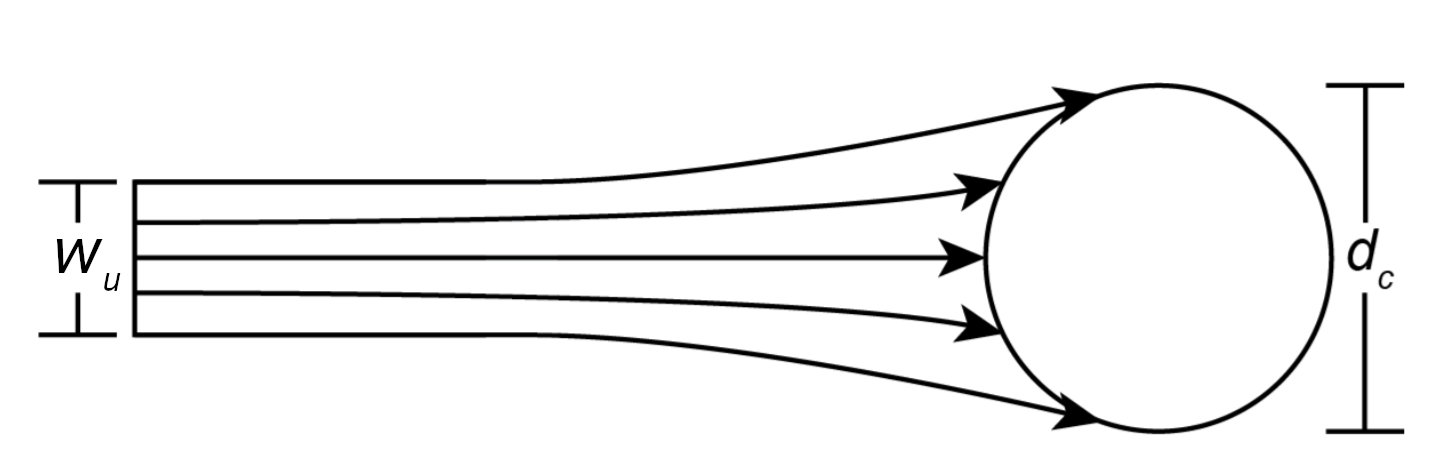
\includegraphics[width=5in]{../pics/collectorefficiency.png}
\centering
\caption{A diagram illustrating capture efficiency for a cylindrical collector. $w_u$ is the horizontal width of upstream flow and $d_c$ is collector diameter. Adapted from Palmer et al. (2004) \cite{Palmer_2004}.}
\label{fig:capeff}
\end{figure}

Physical properties of collectors, particles, and flow environments are all known to affect capture efficiency, though the relative importance of different mechanisms of effect is still being determined. Greater flow velocities ($u$) and larger particle diameters ($d_p$) result in greater direct capture and inertial impaction of particles on stems \cite{Palmer_2004,fuchs1965mechanics}. However, increased $u$ results in increased turbulence---often parameterized by collector Reynolds number ($\Rey_c=\frac{ud_c}{\nu}$), where $\nu$ is kinematic viscosity---which can trap particles in vortices distant from collector surfaces and shear particles off of collectors, resulting in lower ECE. Increased $d_c$ and spatial density of collectors, which we parameterize as solid volume fraction ($\phi_c$), can also result in increased turbulence intensity due to collector wakes, although at sufficiently high densities, decreasing interstitial distance can limit turbulence scale and have a damping effect on turbulent kinetic energy (TKE) \cite{nepf_drag_1999}. Lastly, biofilm comprising algae, cyanobacteria, and other microorganisms that live on the surfaces of submerged vegetation, has been confirmed to affect capture efficiency \cite{Fauria_2015}. Increased stem roughness \cite{Palmer_2004} seems a likely mechanism, along with possibly improved particle adherence \cite{wu2014colloid}.

While analytical expressions have been developed for particle capture in creeping and potential flows \cite{lamb1932, langmuir1942filtration, fuchs1965mechanics}, the complexity of the effects described above precludes theoretical solutions for transitional turbulence (approx: $1<\Rey_c<1000$), which occurs commonly in the environments and on the length scales of aquatic macrovegetation. Hence, empirical estimates are often employed. Palmer \cite{Palmer_2004} introduced a power law expression:

\begin{equation}
    \eta=C{\Rey_c}^{a}R^{b}\,,
    \label{eq:powerlaw}
\end{equation}

\noindent where $C$, $a$, and $b$ are empirically determined regression coefficients. They used an isolated single cylinder coated with grease, for which retention was assumed to be complete ($p_r = 1$), and yielded a model,

\begin{equation}
    \eta=0.224{\Rey_c}^{0.718}R^{2.08}\,,
    \label{eq:palmer}
\end{equation}

\noindent with a $b$ coefficient closer to the analytical expression for creeping flows ($O(R^2)$) than that for potential flows ($O(R)$). Wu et al. \cite{Wu_2011} studied single-collector capture efficiency of colloid particles, which have different physicochemical interactions with collector surfaces, and found a contrasting model:

\begin{equation}
    \eta_0=0.0044{\Rey_c}^{-0.94}N_{\Pec}^{-0.03}\,,
    \label{eq:wu}
\end{equation}

\noindent where $\eta_0$ is contact efficiency, which accounts for $p_r < 1$ due to particles not adhering on initial contact, but still assumes zero resuspension, and $N_{\Pec}$ is the Peclet number ($ud_c/D$, where $D$ is the dispersion coefficient of the sediment). However, because of their study's focus on laminar flow, their model might not scale to transitionally turbulent conditions.

Before our investigation, two other laboratory studies have examined sediment capture in patches of multiple collectors \cite{purich2006capture,Fauria_2015}. Purich \cite{purich2006capture}, who also used greased cylindrical collectors, found a negative relationship between $\eta$ and $\Rey_c$ for their middle collector-density treatment, but little to no effect---and low absolute $\eta$ values---for their high- and low-density treatments. Fauria et al. \cite{Fauria_2015} studied artificial leaves as opposed to stems and yielded a new model for ECE in patches of multiple collectors based on the form of Eq. (\ref{eq:powerlaw}):

\begin{equation}
    \eta^\prime=C{\Rey_c}^{-1.14}R^{0.65}\,,
    \label{eq:fauria}
\end{equation}


\noindent where $C$ varied depending on their other explicative variables: collector density and biofilm. While they did find higher ECE at lower collector density, and with biofilm present, they only estimated two collector-density treatments, and only determined the effect for biofilm for one of the two. Their study design also did not differentiate enhanced gravitational settling theorized to occur in the proximity of collectors from direct capture on their leaves' surfaces. Perhaps most importantly, neither Fauria et al. nor Purich reported the uncertainty of their respective ECE or $\eta$ estimates.

With so many variables differing between relatively few studies, additional experimental work is needed to fill in yet unexplored parameter combinations. For example, Eq. (\ref{eq:fauria}) has only been tested on leaf-shaped collectors as opposed to vertical cylinders, and the synthetic particulate matter used by Purich \cite{purich2006capture} has physical properties well outside the range of sediment expected in most natural settings. Our study builds on previous work by testing Eq. (\ref{eq:fauria}) for cylindrical collectors across a range of $\Rey_c$ similar to Fauria et al \cite{Fauria_2015} and an expanded range of multiple $\phi_c$ values. Additionally, we measure TKE \textit{in situ} to assess its role as a mediator variable between collector density and ECE, delve into the importance of biofilm relative to $\Rey_c$ and $\phi_c$ across a range of collector densities, estimate uncertainty in ECE for our particular experimental conditions, and take the first steps towards a quantitative model for ECE as a function of $\phi_c$.

\section{Materials and Methods}

\subsection{Experimental Methods}

\subsubsection{Materials}

We conducted our experiments in the Ecogeomorphology flume, an indoor (22.2 +/- 1 \SI{}{\celsius}) recirculating flume located in McCone Hall at the University of California, Berkeley. The flume has a rectangular open-channel section (5.25 m L $\times$ 0.6 m W $\times$ 0.6 m H) and a bed and sidewalls that are smooth and transparent (Figure \ref{fig:floorplan}). At its upstream and downstream ends, this section connects to rectangular ducts with gradually changing hydraulic diameter and rounded corners with curved vertical manifolds along streamlines. These features are intended to maintain laminar flow when water is not affected by collectors. Additionally, at the upstream end of the open-channel, a honeycomb flow collimator served to further straighten flow streamlines before water enters the open channel. 

% Flume diagram figure
\begin{figure}[htb]
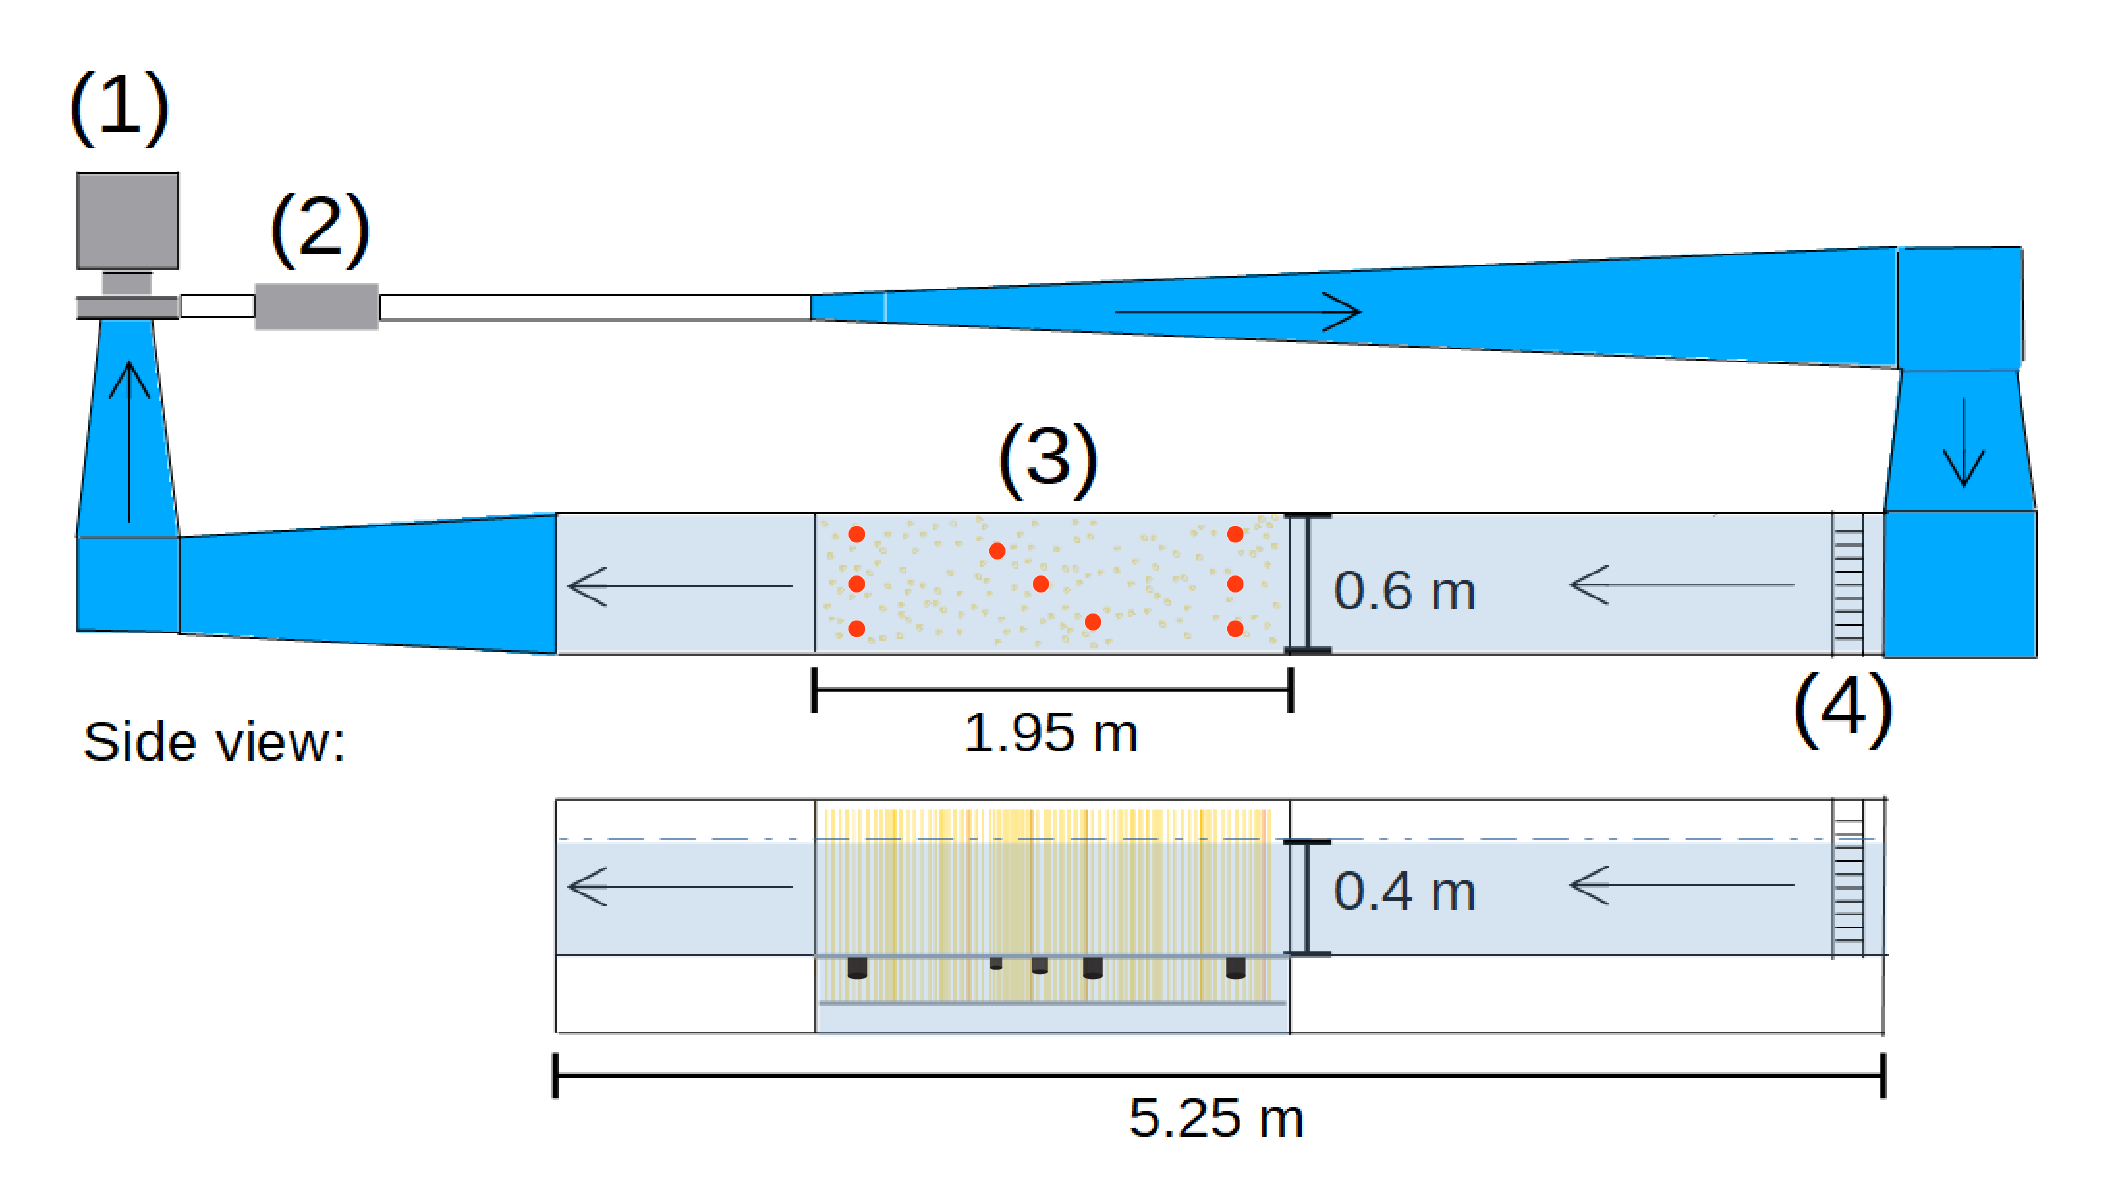
\includegraphics[width=5in]{../pics/flume_with_sedtraps.png}
\centering
\caption{The Ecogeomorphology flume. Not all measurements are to scale. \textbf{(a)} Photograph of the test section (center-left) and pump (right). \textbf{(b)} Conceptual diagram of the flume as seen from above. Labeled parts are: 1) pump, 2) magnetic flowmeter, 3) test section, and 4) honeycomb flow collimator. Arrows indicate direction of flow. Green points represent the inlets for the peristaltic pumps sampling suspended particle concentration. Red areas represent the sediment traps. \textbf{(c)} A side view of the open-channel part of the system.}
\label{fig:floorplan}
\end{figure}

In turn, the ducts guide water to and from the inlet and outlet of the pump array, which consists of a disc pump (Discflo Pumps Corporation, Santee, CA), and a magnetic flowmeter, connected by PVC pipe. This type of pump uses rotating discs to generate viscous drag, which entrains fluid and suspended particles through its interior chamber while maintaining laminar flow and avoiding structural disruption, pulsation, and abrasion \cite{discflo}. Altogether, the flume design maintains constant, adjustable discharge through the open channel, minimizing background turbulence and other artifacts that arise with other types of pumps.

Within the open channel, we designated a "test section" 1.95 m in length where collectors would be installed. This test section and the surrounding area were instrumented with the following devices:
\begin{enumerate}
     \item A flat-bedded array positioned flush with the neighboring channel bed, containing vertical, emergent collector stems, which were spaced uniformly in an unpatterned manner
    \item Two battery-operated peristaltic pumps (Cole-Parmer, Vernon Hills, IL) used to sample suspended particle concentration via three hose inlets each (inside diameter = 3.1 mm), which were suspended at a range of heights from the channel bed (5; 14; 27 cm); these were positioned 50 cm upstream and downstream of the test section 
   \item sediment traps (n = 9) with 2.5 cm circular openings flush with the bed and collection filters (Whatman GF/F) on perforated filter holders recessed in a 5 cm deep cylindrical cavity (trap Reynolds number and aspect ratio chosen to minimize bias \cite{butman1986sediment}); these were interspersed among the collectors in a grid-like pattern
\end{enumerate}

We used 1/8" (0.3175 cm) cylindrical wooden dowels as collectors, which were covered in silicone grease (Chemplex 710, Fuchs Petrolub, Mannheim, Germany) in order to retain impacted particles and spread randomly throughout the test section at the appropriate density. Crushed walnut shell was used as a substitute for suspended sediment because it has surficial and physical properties comparable to the organic-rich types common in wetlands \cite{muller2017experiments, jenzer2015sediment, redding2006particle}. We used WF5-200 grade (Composition Materials Co., Milford, CT), which passes entirely through a \#60 sieve (\SI{250}{\micro\metre}), and which we determined has a average particle diameter ($d_{50}$) of \SI{25.2}{\micro\metre} based on measurements using a laser-scattering-based instrument (LISST-Portable|XR, Sequoia Scientific, Bellevue, WA; See Appendix A1). We also empirically estimated the particle density for this specific walnut shell flour to be 1.53 \SI{}{\gram/\centi\metre\cubed} using volume displacement.

\subsubsection{Suspended Particle Concentration Analysis}

We conducted experimental runs for a fully-crossed parameter space of collector Reynolds number (67; 134; 200) and collector density (0; 285; 821; 1487 collectors/m$^2$ bed area). These values, as well as other experimental parameters held constant throughout, were chosen because they correspond to those that might occur for emergent grasses or reeds in natural settings (Table \ref{tbl:parameters}). A zero-collector control density was included in order to isolate the effects of our experimental installations from the background effects of the rest of the flume.   

% Experimental parameters table
\begin{table}[h]
\caption{Experimental and natural parameter ranges. Natural values are based on approximations or measurements from cited studies and literature reviews in wetlands or other low-elevation flows.}
\centering
\begin{threeparttable}
\begin{tabular}{lcccc}
\toprule
\textbf{Parameter}&\textbf{This study}&\textbf{Fauria et al. (2015)}&\textbf{Purich (2006)}&\textbf{Natural}\\
\midrule
Flow velocity (\SI{}{\centi\metre/\second})     
& 2.0--6.0    & 1.8--6.1    & 1.0--10.2    & 0--25 \cite{nikora2008hydraulic}    \\
Flow depth (\SI{}{\centi\metre})                
& 40          & 14--17      & 12           & 0--50 \cite{kadlec1990}    \\
\midrule
Collector shape
& Cylindrical & Artificial grass  & Cylindrical & Varies \\ 
Collector diameter (\SI{}{\centi\metre})
& 0.318       & 0.3         & 0.6          & 0.1--1.2 \cite{Nepf_2012,wright2018hydrological} \\
Collector Reynolds number                       
& 66--200     & 54--183     & 70--640      & 5--1000 \cite{kadlec1990}  \\ 
Collector density ($\#/\text{m}^2$)
& 285--1487   & 2724--7209  & 1013--4053   & 10--2700 \cite{wright2018hydrological} \\
Solid volume fraction (\%)
& 0.22--1.17  & 0.82--2.16  & 2.86--11.5   & 0.1--1 \cite{Nepf_2012}   \\ 
\midrule
Particle type
& Walnut shell  & Road dust  & Pliolite\textsuperscript{\textregistered}   & Sediment \\ 
Particle density  (\SI{}{\gram/\centi\metre\cubed})    
& 1.53        &2.27--2.61 \tnote{1}  & 1.03         & 1.43--2.39 \cite{redding2006particle} \\
Average particle diameter, $d_{50}$ (\SI{}{\micro\metre})     
& 25.2        & $\sim$10--15 \tnote{2} & 212--250     & 45--100 \cite{hejduk2010variations,noe2010glades}  \\
Suspended concentration (\SI{}{\micro\liter/\liter})      
& 5--55   & <9--50 \tnote{2}      & $\sim$110   & 2-25 \cite{noe2010glades,aiona2013can}      \\
\midrule
Particle-collector diameter ratio, $R$      
&0.0079       &0.0004--0.083 \tnote{2} & 0.037        & <0.25     \\
\bottomrule
\vspace{-4mm}
\end{tabular}
\begin{tablenotes}
\footnotesize \item[1] Estimated from a different study about road dust properties \cite{mckenzie2008size} 
\vspace{2mm}
\footnotesize \item[2] Fauria et al. \cite{Fauria_2015} used a LISST to measure capture in separate bins across a broad range of particle diameters (1.25--250 \SI{}{\micro\metre}) rather than overall suspended concentration
\end{tablenotes}
\end{threeparttable}
\label{tbl:parameters}
\end{table}

Before each experiment, the flume was filled with tap water to 0.4 m depth in the test section, which was enough to fully submerge the pump and almost the entirety of the duct length. At this depth, the volume of water in the entire flume was approximately 2.43 m$^3$ (See Appendix A2).  A Nortek Vectrino Profiler ADV (acoustic Doppler velocimeter; Nortek AS, Vangkroken 2, 1351 Rud, Norway) was used to calibrate the pump to generate channel mean flow velocities (2.0; 4.0; 6.0 \SI{}{\centi\metre/\second}) within the pump's capabilities and corresponding to the range of interest for $\Rey_c$. At these flow rates (0.0048; 0.0096; 0.0144 \SI{}{\metre\cubed/\second}), circulation times for the entire system were 506 s, 253 s, and 169 s, respectively. The drag caused by collectors was not found to detectably affect upstream or downstream flow velocities.

Sediment traps were installed immediately before each run, then a slurry consisting of 200 g of crushed walnut shell suspended in 15.1 L of tap water was added using a spigot calibrated to finish draining after a period roughly equal to circulation time (3 minutes). Test-section flow velocity was kept at 6 cm/s for this period across $\Rey_c$ treatments, then adjusted to the appropriate value for the treatment. This procedure was intended to make particle concentration longitudinally even throughout the system. Estimated depth-averaged starting concentration was 82.3 mg/L (\SI{53.8}{\micro\liter/\liter}).

In preliminary experiments, we determined 100 minutes was more than adequate to capture the effects of settling and capture on suspended concentrations across our parameter space. We sampled suspended concentration using the peristaltic pumps every 5 minutes, the first sample occurring 5 minutes after we began adding sediment to the flume. Samples measured approximately 140 ml each, and our sampling frequency resulted in 19 sampled timesteps per experiment, with six samples per timestep. sediment traps were covered with a plunger and removed at 100 minutes, so the last peristaltic pump sample occurred at 95 minutes due to personnel limitations.

Peristaltic pump samples were processed using vacuum filtration. Before filtration, quantitative glass microfiber filter papers (Whatman GF/F) were oven-dried for 24 hours at \SI{40}{\celsius} to remove any moisture, weighed, and assigned to a flume sample. The volume of flume water passed through the filter was measured, then the drying and weighing process was repeated to estimate the mass of sediment on the filter. Concentrations were recorded in \SI{}{\milli\gram/\liter}. Filter papers from sediment traps were dried and weighed before and after the run in a similar fashion, to estimate the mass of settled particles they contained.

\subsubsection{Estimating Collector-Induced Turbulence}

We estimated mid-water-column turbulent kinetic energy (TKE) among the collectors for each combination of $\Rey_c$ and collector density using the Vectrino Profiler ADV. The Vectrino was mounted on a frame suspended above the test section and adjusted until its bottom-depth measurement read 15 cm. A bubble level was used to ensure it was oriented along the vertical axis. The ADV measured velocity in two horizontal dimensions, and two separate measurements along the vertical dimension, at a frequency of 10 Hz. It also collected other data such as autocorrelation and signal-to-noise ratio. We collected 5 minutes of data per treatment in the interest of including the vast majority of expected periodicity in our variance measurement. Measurements taken by the ADV were filtered, leaving out timepoints where the two vertical velocity measurements differed by 50\% or more or the SNR measurement was greater than 5 dB, and were subsequently despiked using a phase-space thresholding algorithm \cite{goring_nikora}. TKE was derived from the cleaned Vectrino data as half the sum of the variances of the velocity components:
\begin{equation}
    \text{TKE} = \frac{1}{2}[\overline{(u^\prime)^2} + \overline{(v^\prime)^2} + \overline{(w^\prime)^2}]\,.
    \label{eqn:TKE}
\end{equation}

\subsubsection{Biofilm Growth}

The effect of biofilm on the surficial properties of collectors, and thereby their effective capture efficiency, was another factor of interest for our experiment. While we did not incorporate biofilm into the fully-crossed parameter space of other explicative variables due to the time-intensiveness of growing algae, we did carry out an auxiliary experiment to roughly assess its effect size. After one of the experiments at each collector density, the water in the flume was allowed to come to rest, then the collectors sat constantly illuminated by one white, fluorescent grow-light for a measured number of days. The crushed walnut shell doubled as a food source for the microorganisms constituting the biofilm, which we observed grew plentifully in all cases.

Once biofilm became visually apparent on the collectors' surfaces, an experiment was conducted using the same materials and protocols as the treatments without biofilm, holding $\Rey_c = 200$ constant between biofilm treatments. The length of time it took for robust biofilm growth to occur differed between the low, medium, and high collector-density treatments (13; 18; 20 days, respectively). For the highest collector-density treatment, a follow-up experiment with a longer growth period (46 days) was performed. While we did not quantitatively assess biofilm mass, we assumed that the number of days it was allowed to grow could be used as a proxy, acknowledging that the growth rate (in mass units per day) was probably exponential or logistic rather than linear.

\subsection{Sediment Transport and Particle Capture Model}

\subsubsection{Model Derivation}

We used an exponential decay model for suspended sediment concentration adapted from Fauria et al. \cite{Fauria_2015} to estimate ECE ($\eta^\prime$):

\begin{equation}
    \frac{\mathrm{d}\bar{\phi}}{\mathrm{d}t} = -\left[\frac{C_bv_s}{h}(1-E_r) + \eta^{\prime}ud_cI_c\right]\bar{\phi}(t) = -(k_s + k_c)\bar{\phi}(t) = -k\bar{\phi}(t)\,.
    \label{eq:model}    
\end{equation}

\noindent $\bar{\phi}(t) = \frac{1}{h} \int_0^h\phi(z) \,\mathrm{d}z$ is the depth-averaged suspended sediment concentration at time $t$, where $h$ is water depth, $z$ is height above the bed, and $\phi(z)$ is concentration at height $z$. $k_s = \frac{C_bv_s}{h}(1-E_r)$ is the exponential time-decay rate of $\bar{\phi}$ due to settling, which is calculated from settling velocity ($v_s$), $h$, a constant ($C_b$) that accounts for the concentration near the bed predicted by the Rouse equation relative to $\bar{\phi}$, and a dimensionless rate at which particles are entrained from the bed ($E_r$). Further derivation of $k_s$ is available in Fauria et al. \cite{Fauria_2015}. $k_c$ = $\eta^{\prime}ud_cI_c$ is the rate at which particles are removed from suspension due to capture by collectors. $I_c = \frac{N_ch}{V}$ is collector height density, where $N_c$ is the total number of stems, and $V$ is the volume of water in which stems are contained.

The solution of the differential equation (Eq. (\ref{eq:model})) is exponential,

\begin{equation}
    \bar{\phi}(t) = \bar{\phi}(0)e^{-kt} = \bar{\phi}(0)e^{-(k_s + k_c)t}\,.
    \label{eq:expo}    
\end{equation}

\noindent Concentration at any height can be assumed to change over time in proportion to average concentration because we assume the vertical profile of sediment concentration maintains a constant shape governed by the Rouse equation \cite{rouse1937modern},

\begin{equation}
    \frac{\phi_z}{\phi_r} = \left( \frac{h - z}{z} \frac{z_r}{h - z_r} \right)^{R_0}\,,
    \label{eq:rouse}    
\end{equation}

\noindent where $\phi_r$ is concentration at an arbitrary reference height above the bed ($z_r$), conventionally $0.05h$, and $R_0$ is referred to as the Rouse number \cite{kumbhakar2017derivation}.

To calculate $k_s$, we began by calculating the average mass of sediment that settled per sediment trap over the duration of the experiment (100 minutes). We then scaled this measurement up from the area of a sediment trap's horizontal opening (5.07 $\times 10^{-4}$ m$^2$) to the total test section bed area (1.17 m$^2$). The resulting estimate of the sediment mass settled in the test section ($m_s$) was divided by the total mass removed from suspension during a run to calculate the proportion of the decrease due to settling. This proportion was multiplied by the total exponential decay coefficient, $k$, to calculate $k_s$:

\begin{equation}
    k_s = \frac{m_s}{m_0(1-e^{-kT})}k\,,
    \label{eq:ks}
\end{equation}

\noindent where $m_0$ was the mass of sediment suspended at the beginning of the experiment and $T$ was the total duration of the experiment.

The equations above model the dynamics occurring in the test section alone. To account for settling and reentrainment outside the test section, a background exponential decay rate ($k_b$) was estimated from runs with zero collectors for each $\Rey_c$ treatment ($k_c = 0 \implies k_b = k - k_s$). ECE for our collector-density treatments was then calculated from $k_c$. Also, because collectors only act on suspended particles while they are passing through the test section, this estimate for ECE was scaled by the ratio (5.19) between the total volume of water in the flume (\SI{2.43}{\metre\cubed}) and $V = \SI{0.468}{\metre\cubed}$:

\begin{equation}
    \eta^\prime = 5.19\frac{k_c}{ud_cI_c} = 5.19\frac{k - k_s - k_b}{ud_cI_c}\,.
    \label{eq:eta}
\end{equation}

\subsubsection{Model Execution}

In order to correct for observed heteroscedasticity (See Appendix A3) across time, with earlier, higher-concentration measurements showing greater variance, we log-transformed the exponential model (Eq. (\ref{eq:expo})). This resulted in a linear model taking the form,

\begin{equation}
    log(\boldsymbol{\bar{\phi}}) = log(\bar{\phi}(0)) - k\boldsymbol{t} + \boldsymbol{U} \,,
\end{equation}

\noindent which was evaluated for each experimental configuration separately. Bold font signifies vector variables, and $\boldsymbol{U}$ is the random error term of the model. The standard error of this $k$ term and the standard deviation of $m_s$ estimates from sediment traps were propagated through Eqs. (\ref{eq:ks}) and (\ref{eq:eta}), for both control and treatment runs, and were ultimately used to calculate uncertainty estimates for ECE.

Our experiment collected suspended concentration samples at three different heights and both upstream and downstream of the test section. Because the observed magnitude of the Rouse profile (Eq. (\ref{eq:rouse})) and the upstream-downstream difference were barely detectable with our degree of precision, and both were negligible relative to the concentration decay over time, we opted to pool data from all six suspended sediment sampling locations rather than complicating the model further. While we might overestimate or underestimate absolute concentration this way, exponential decay is expected to be constant across height on account of the constant Rouse profile, and thus estimated ECE would not be affected.

We used a Monte Carlo approach to assess the significance of the effects of $\Rey_c$ and $\phi_c$ on ECE. For each combination of $\Rey_c$ and $\phi_c$, 30,000 random values were drawn from a normal distribution whose mean equals that combination's empirically estimated ECE and whose standard deviation equals its standard error (SE). These values were log-transformed, since we expected the relationships to fit a power-law model. For each stratum of a given explicative variable, sets (triplets) with one randomly sampled value from each of the strata of the other explicative variable were regressed using ordinary least squares, producing a roughly normal distribution of coefficients (n = 30,000) for each level of both variables (6 total). The distributions of slopes were used in two-tailed t-tests (null hypothesis: $\mu = 0$; $\alpha = 0.05$) to determine the significance of relationships.

Lastly, we compared our results to Fauria et al. \cite{Fauria_2015} by fitting their model (Eq. (\ref{eq:fauria})) to our data at each of our collector densities, estimating $C$, then fitting a power-law function relating the combined $C$ values from their study and ours to collector density. $C$ is directly proportional to ECE in their model, so this can be thought of as an indirect way to quantify the relationship between collector density and ECE.

\section{Results}

\subsection{Particle Capture}

Effective capture efficiency was found to decrease with increasing $\Rey_c$ and $\phi_c$ throughout our parameter space, with one exception. This exception occurred at the lowest collector density ($\phi_c = 0.22\%$), where the intermediate $\Rey_c$ treatment ($\Rey_c = 134$) had lower ECE than both the lower and higher $\Rey_c$ treatments (Figure \ref{fig:ece}a). When compared to the other collector-density treatments with the same $\Rey_c$ value, this low collector-density experiment's calculated ECE was slightly lower than the intermediate collector-density treatment, and was greater than the highest collector-density treatment (Figure \ref{fig:ece}b). Our experimental uncertainty was great enough that this might be attributable to random error. However, repeating the experiment with the same parameters yielded a nearly identical result (omitted from analysis).

% ECE figure
\begin{figure}[htb]
\centering
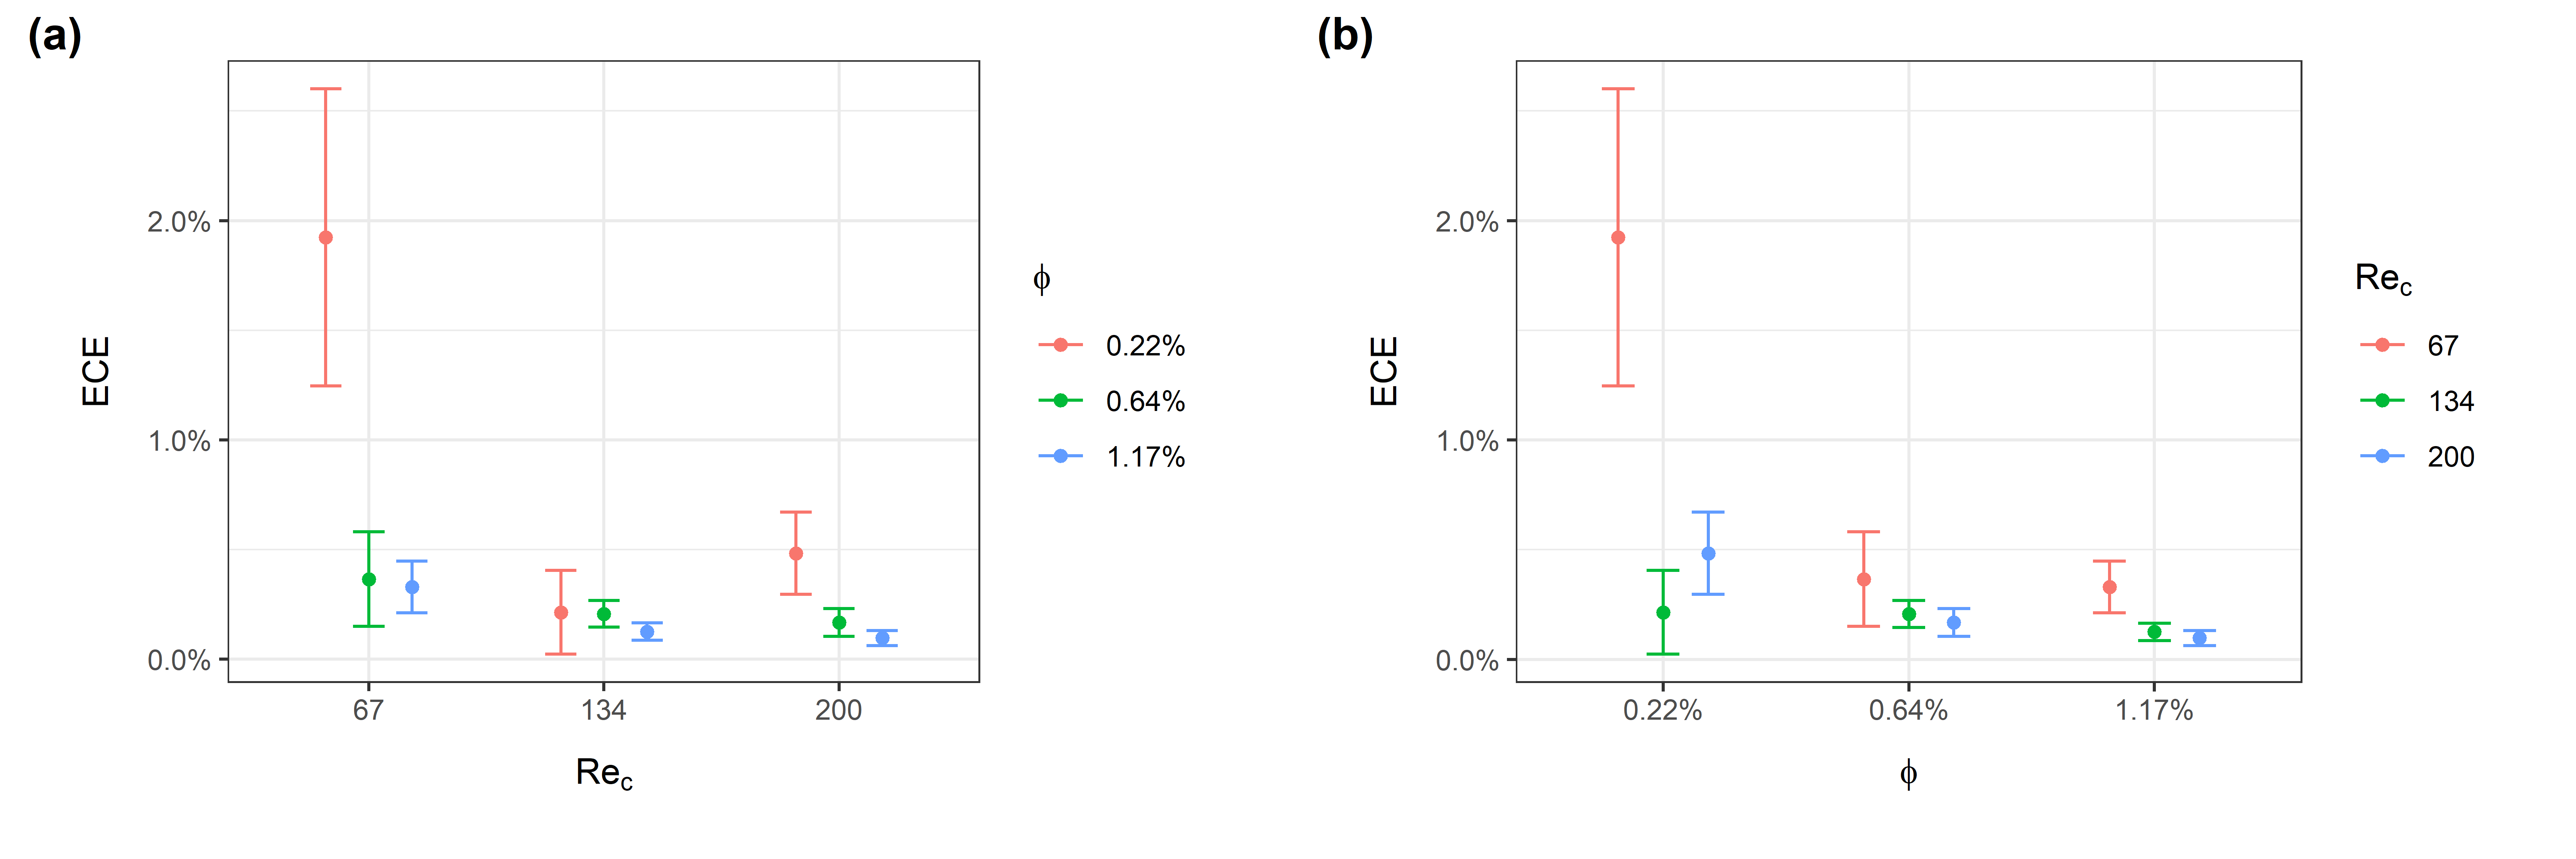
\includegraphics[width=5in]{../pics/ece_plot.png}
\caption{Estimates of effective capture efficiency calculated from laboratory experiments across the collector density $\times$ Reynolds number ($\Rey_c$) parameter space. Error bars represent +/- 1 SE. (\textbf{a}) Estimates plotted over $\Rey_c$, colored by solid volume fraction ($\phi_c$). (\textbf{b}) Estimates plotted over $\phi_c$, colored by $\Rey_c$.}
\label{fig:ece}
\end{figure}   

Monte Carlo analysis determined that there is a significant negative relationship between ECE and collector density for the low (p = 0.004) and high (p = 0.019) $\Rey_c$ treatments, but no significant effect was detected (p > 0.05) for the intermediate treatment (Figure \ref{fig:monte}a). We also found a significant negative relationship between ECE and $\Rey_c$ for the low (p = 0.026) and high (p = 0.046) collector-density treatments, but an insignificant (p > 0.05) trend for the intermediate collector-density treatment (Figure \ref{fig:monte}b). 

% Monte Carlo figure
\begin{figure}[H]
\centering
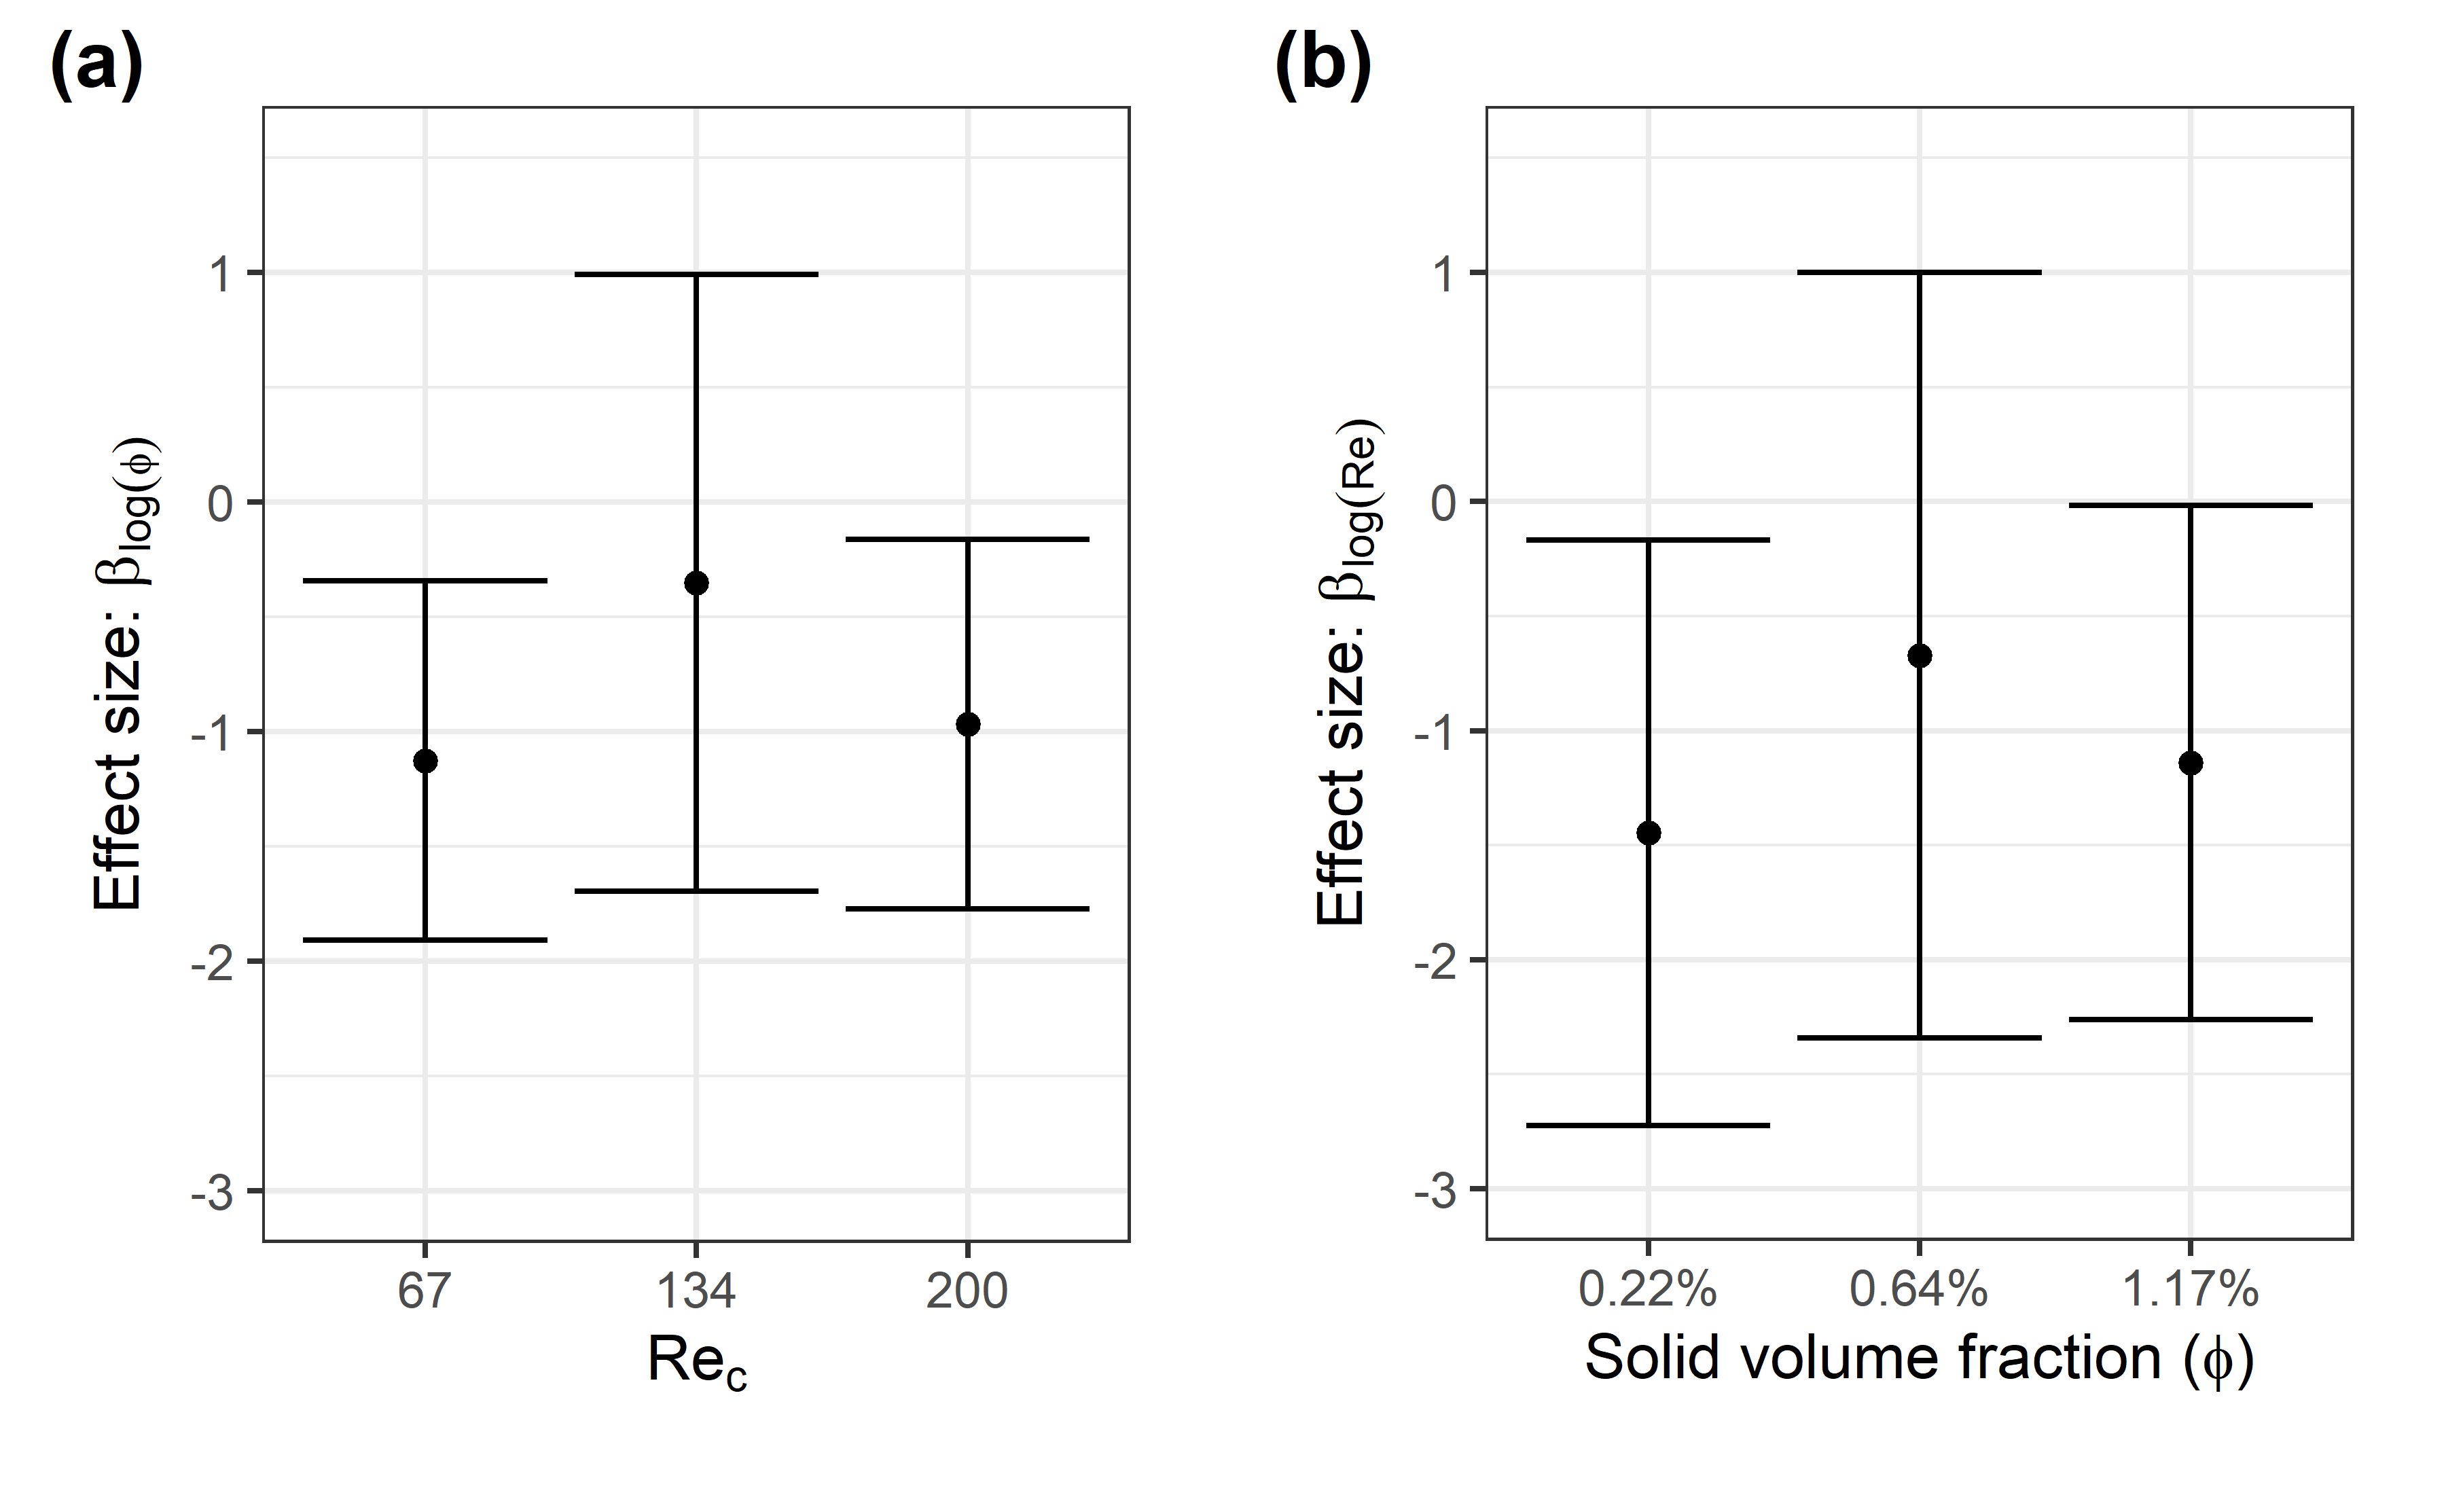
\includegraphics[width=5in]{../pics/montecarlo.png}
\caption{Effect size estimates from Monte Carlo regression analysis. Error bars represent 95\% confidence intervals. Asterisks mark the parameter values at which the effect size was found to be significant. (\textbf{a}) Estimates of the effect of log-transformed collector solid volume fraction ($\beta_{\log(\phi_c)}$) on ECE, stratified by $\Rey_c$. (\textbf{b}) Estimates of the effect of log-transformed $\Rey_c$ ($\beta_{\log(\Rey_c)}$) on ECE, stratified by solid volume fraction ($\phi_c$).}
\label{fig:monte}
\end{figure}   

\subsection{Turbulence}

TKE was consistently found to increase with increasing flow velocity as expected (Table \ref{tbl:turbulence}). Generally, higher collector density also led to greater turbulence, with the greatest increase in terms of both absolute and relative magnitude taking place between the lower and middle collector-density treatments. A slight decrease actually occurred thereafter (between the middle and highest collector densities) for the middle and highest $\Rey_c$ treatments, with a slight increase for the lowest $\Rey_c$ treatment. The similarity of TKE for the upper two collector-density treatments suggests a potential threshold occurring before or near the middle treatment's $\phi_c$ value. ECE and TKE exhibited a negative relationship across the experimental parameter space (n = 9) taken as a whole (Figure \ref{fig:tke}).

% Turbulence table
\begin{table}[H]
\caption{Turbulent kinetic energy (TKE) for all collector solid volume fraction ($\phi_c$) and $\Rey_c$ treatments, including the control (zero-collector) treatments for reference.}
\centering
%% \tablesize{} %% You can specify the fontsize here, e.g., \tablesize{\footnotesize}. If commented out \small will be used.
\begin{tabular}{>{\bfseries}r>{\bfseries}rrr}
\toprule
\textbf{$\phi_c$}&\textbf{$\Rey_c$}&\textbf{mid-water-column TKE (\SI{}{\milli\metre^2/\second^2})}\\
\midrule
Control &   67  & \num{2.48}\\
        &   134 & \num{2.98}\\
        &   200 & \num{3.37}\\
\midrule
0.22\% &   67  & \num{1.23}\\
        &   134 & \num{5.26}\\
        &   200 & \num{12.2}\\
\midrule
0.64\% &   67  & \num{9.13}\\
        &   134 & \num{35.9}\\
        &   200 & \num{59.6}\\
\midrule
1.17\%  &   67  & \num{11.1}\\
        &   134 & \num{29.8}\\
        &   200 & \num{54.4}\\
\bottomrule
\label{tbl:turbulence}
\end{tabular}
\end{table}

\begin{figure}[H]
\centering
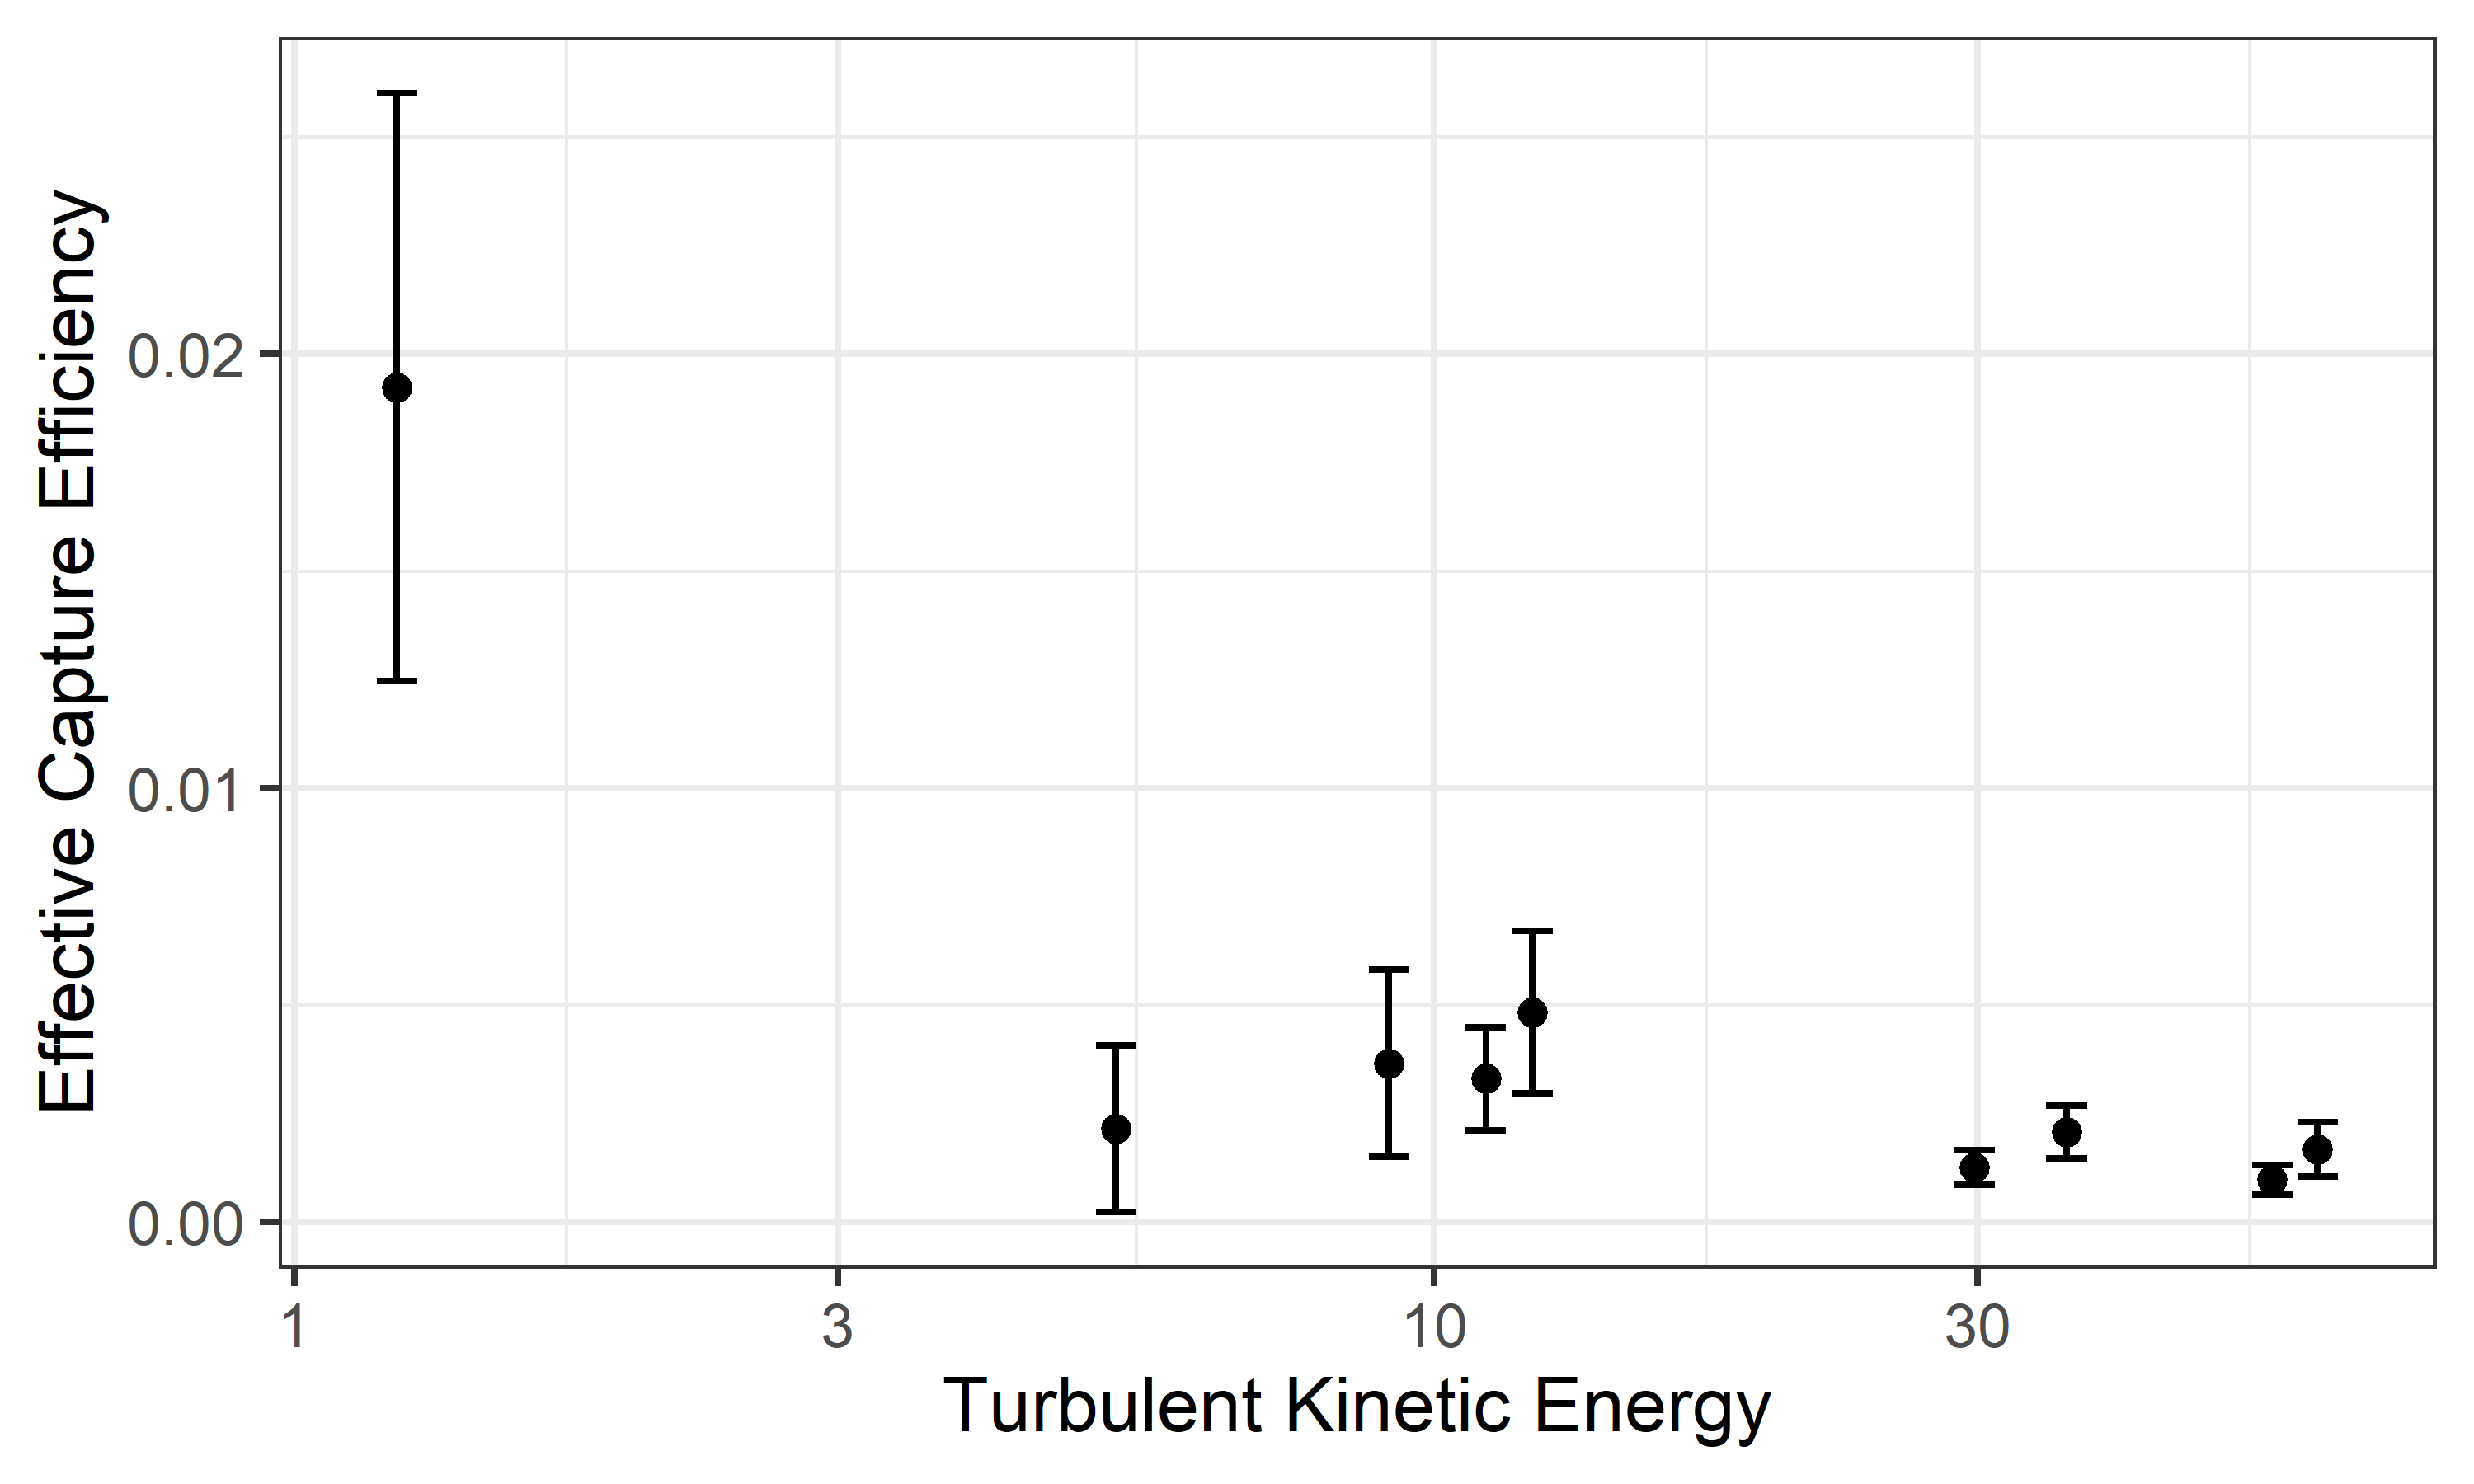
\includegraphics[width=4in]{../pics/tke.png}
\caption{Effective capture efficiency as a function of turbulent kinetic energy for all experimental treatments studied.}
\label{fig:tke}
\end{figure}   

\subsection{Biofilm Effects}

We observed robust biofilm growth, consistent throughout the test section. Biofilm grew on the surfaces of collectors and, as we discovered after turning the pump on, in strands (less than 5 cm long) that were pulled downstream by the flow. Biofilm growth was consistently found to increase ECE (Figure \ref{fig:biofilm}). For the runs conducted when biofilm was first observed to be abundant in the test section (13-20 days), both absolute (+0.71\% ECE) and relative (an improvement to 2.48 times control) increase were greatest by a considerable margin at the lowest collector density, which also had the shortest growth period (13 days). The middle and highest collector densities were fairly close in terms of absolute increase (+0.09\% ECE and +0.07\% ECE, respectively) and relative increase (1.53 times and 1.73 times, respectively). Interestingly, in our test of a longer grow time (46 days) at the highest collector density, ECE increased with far greater relative (7.15 times) and absolute (+0.60\% ECE) magnitude, suggesting that the other runs might not have been at saturation in terms of biofilm mass.

% Biofilm figure
\begin{figure}[H]
\centering
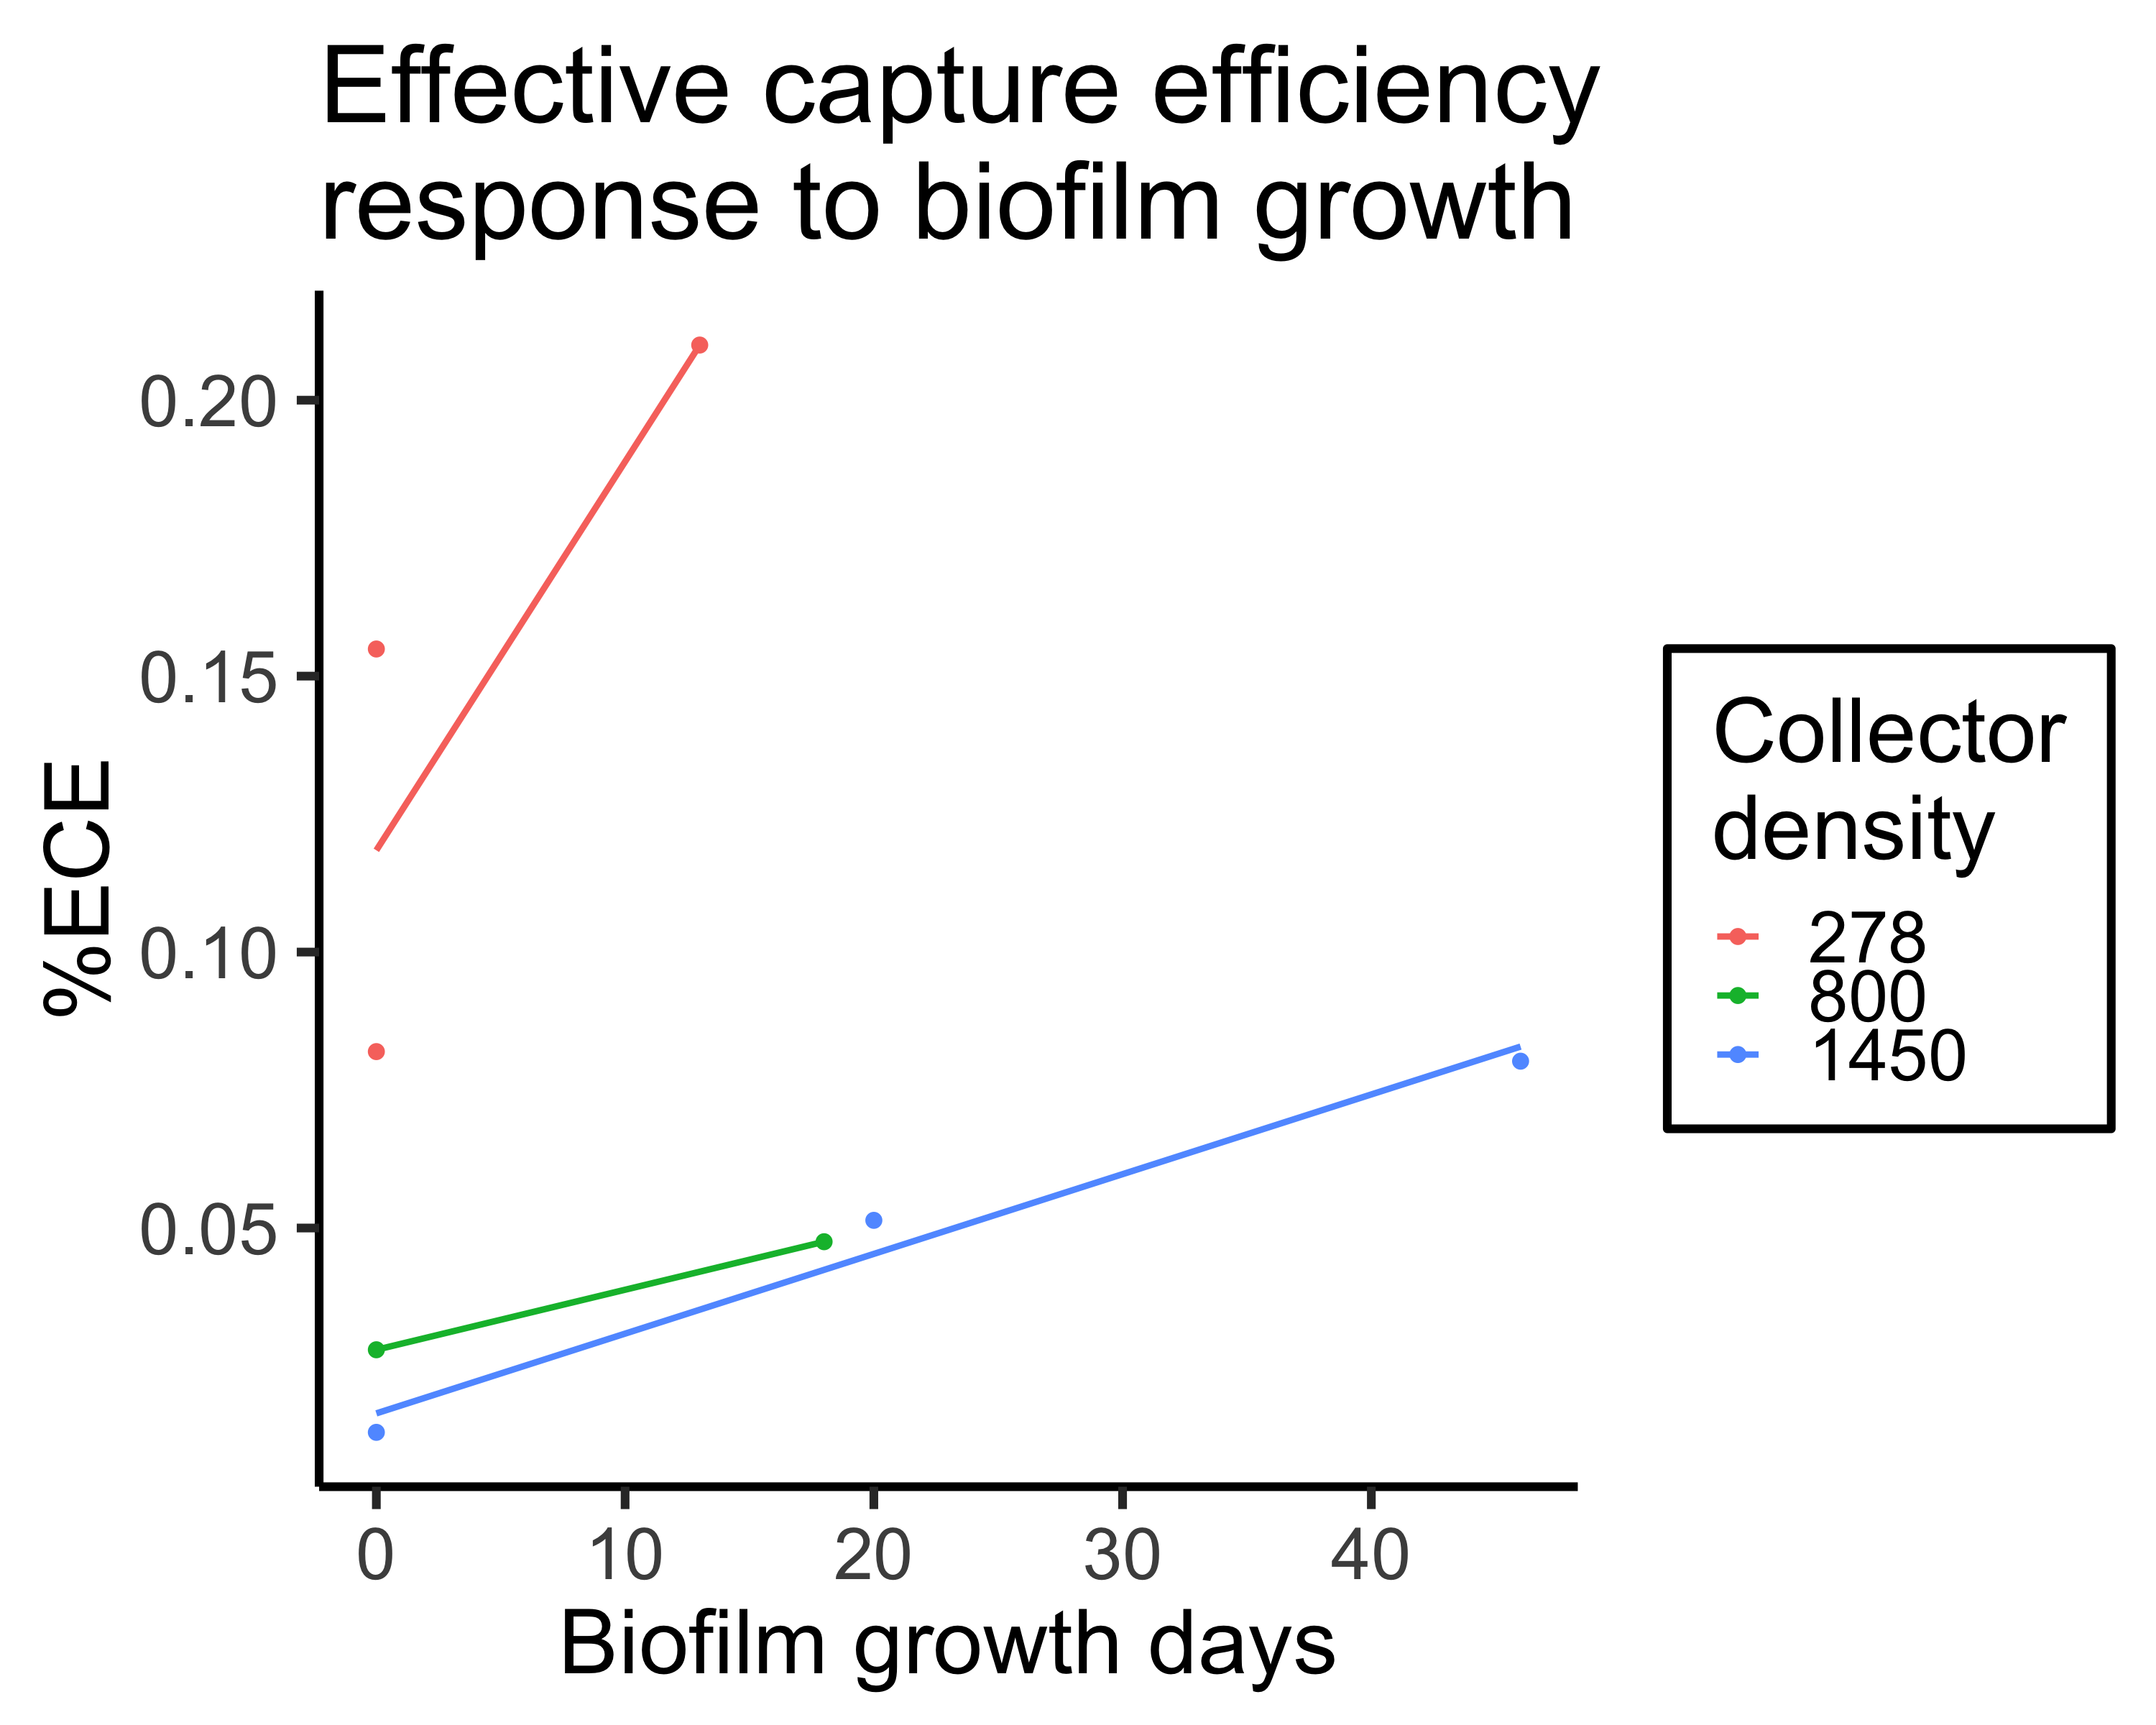
\includegraphics[width=5in]{../pics/biofilm.png}
\caption{Estimates of effective capture efficiency calculated from experimental runs with varying degrees of biofilm growth. Colors represent the different collector densities, expressed as solid volume fraction ($\phi_c$). Straight lines are drawn between the points that represent our experiments and the shaded areas represent 95\% confidence intervals for ECE inferred from our measurement uncertainty.}
\label{fig:biofilm}
\end{figure}   

\subsection{Comparison to Previous Models of Capture Efficiency}

Aside from the outlier at the mid $\Rey_c$, lowest collector-density treatment, all of our observations were in agreement with the power-law model from Fauria et al. \cite{Fauria_2015} (Figure \ref{fig:compplot}). In no other case did the model prediction differ from our empirical observation by more than 1 standard error (SE). Moreover, the model relating $C$ to $\phi_c$ yielded marginally good fit (R$^2$ = 0.82; Figure \ref{fig:cphi}):

\begin{equation}
    C = 0.00801{\phi_c}^{-1.41}\,.
    \label{eq:cphi}
\end{equation}

\noindent It underestimated $C$ for all of our collector-density treatments, and overestimated it for both of those from Fauria et al. ($\phi_c$ = 0.82\%, 2.16\%). However the magnitude of this error was small in comparison to the absolute differences in $C$ among the various $\phi_c$ values (n = 5). Data scarcity should be considered a limiting factor in the interpretation of these results.



\section{Discussion}

\subsection{Inferred Mechanisms of Effect for Collector Density and Reynolds Number}

It is notable that the exponential coefficient for $\phi_c$ as a predictor of $C$ (Eq. (\ref{eq:cphi})), and thus indirectly ECE, is greater in magnitude than those found by Fauria et al. \cite{Fauria_2015} for either $\Rey_c$ or $R$ as a direct predictor of ECE. With the evidence of a positive---albeit potentially thresholded---effect of collector density on TKE, and the evidence of TKE's negative effect on ECE, it seems likely that secondary turbulence generated by upstream collectors negatively affects downstream collectors' ECE. This is conceptually valid because greater fluctuations in flow velocity exert stronger forces with more variable directionality on sediment particles affixed to collectors, increasing the probability of resuspension. 

% Fauria model comparison figure
\begin{figure}[H]
\centering
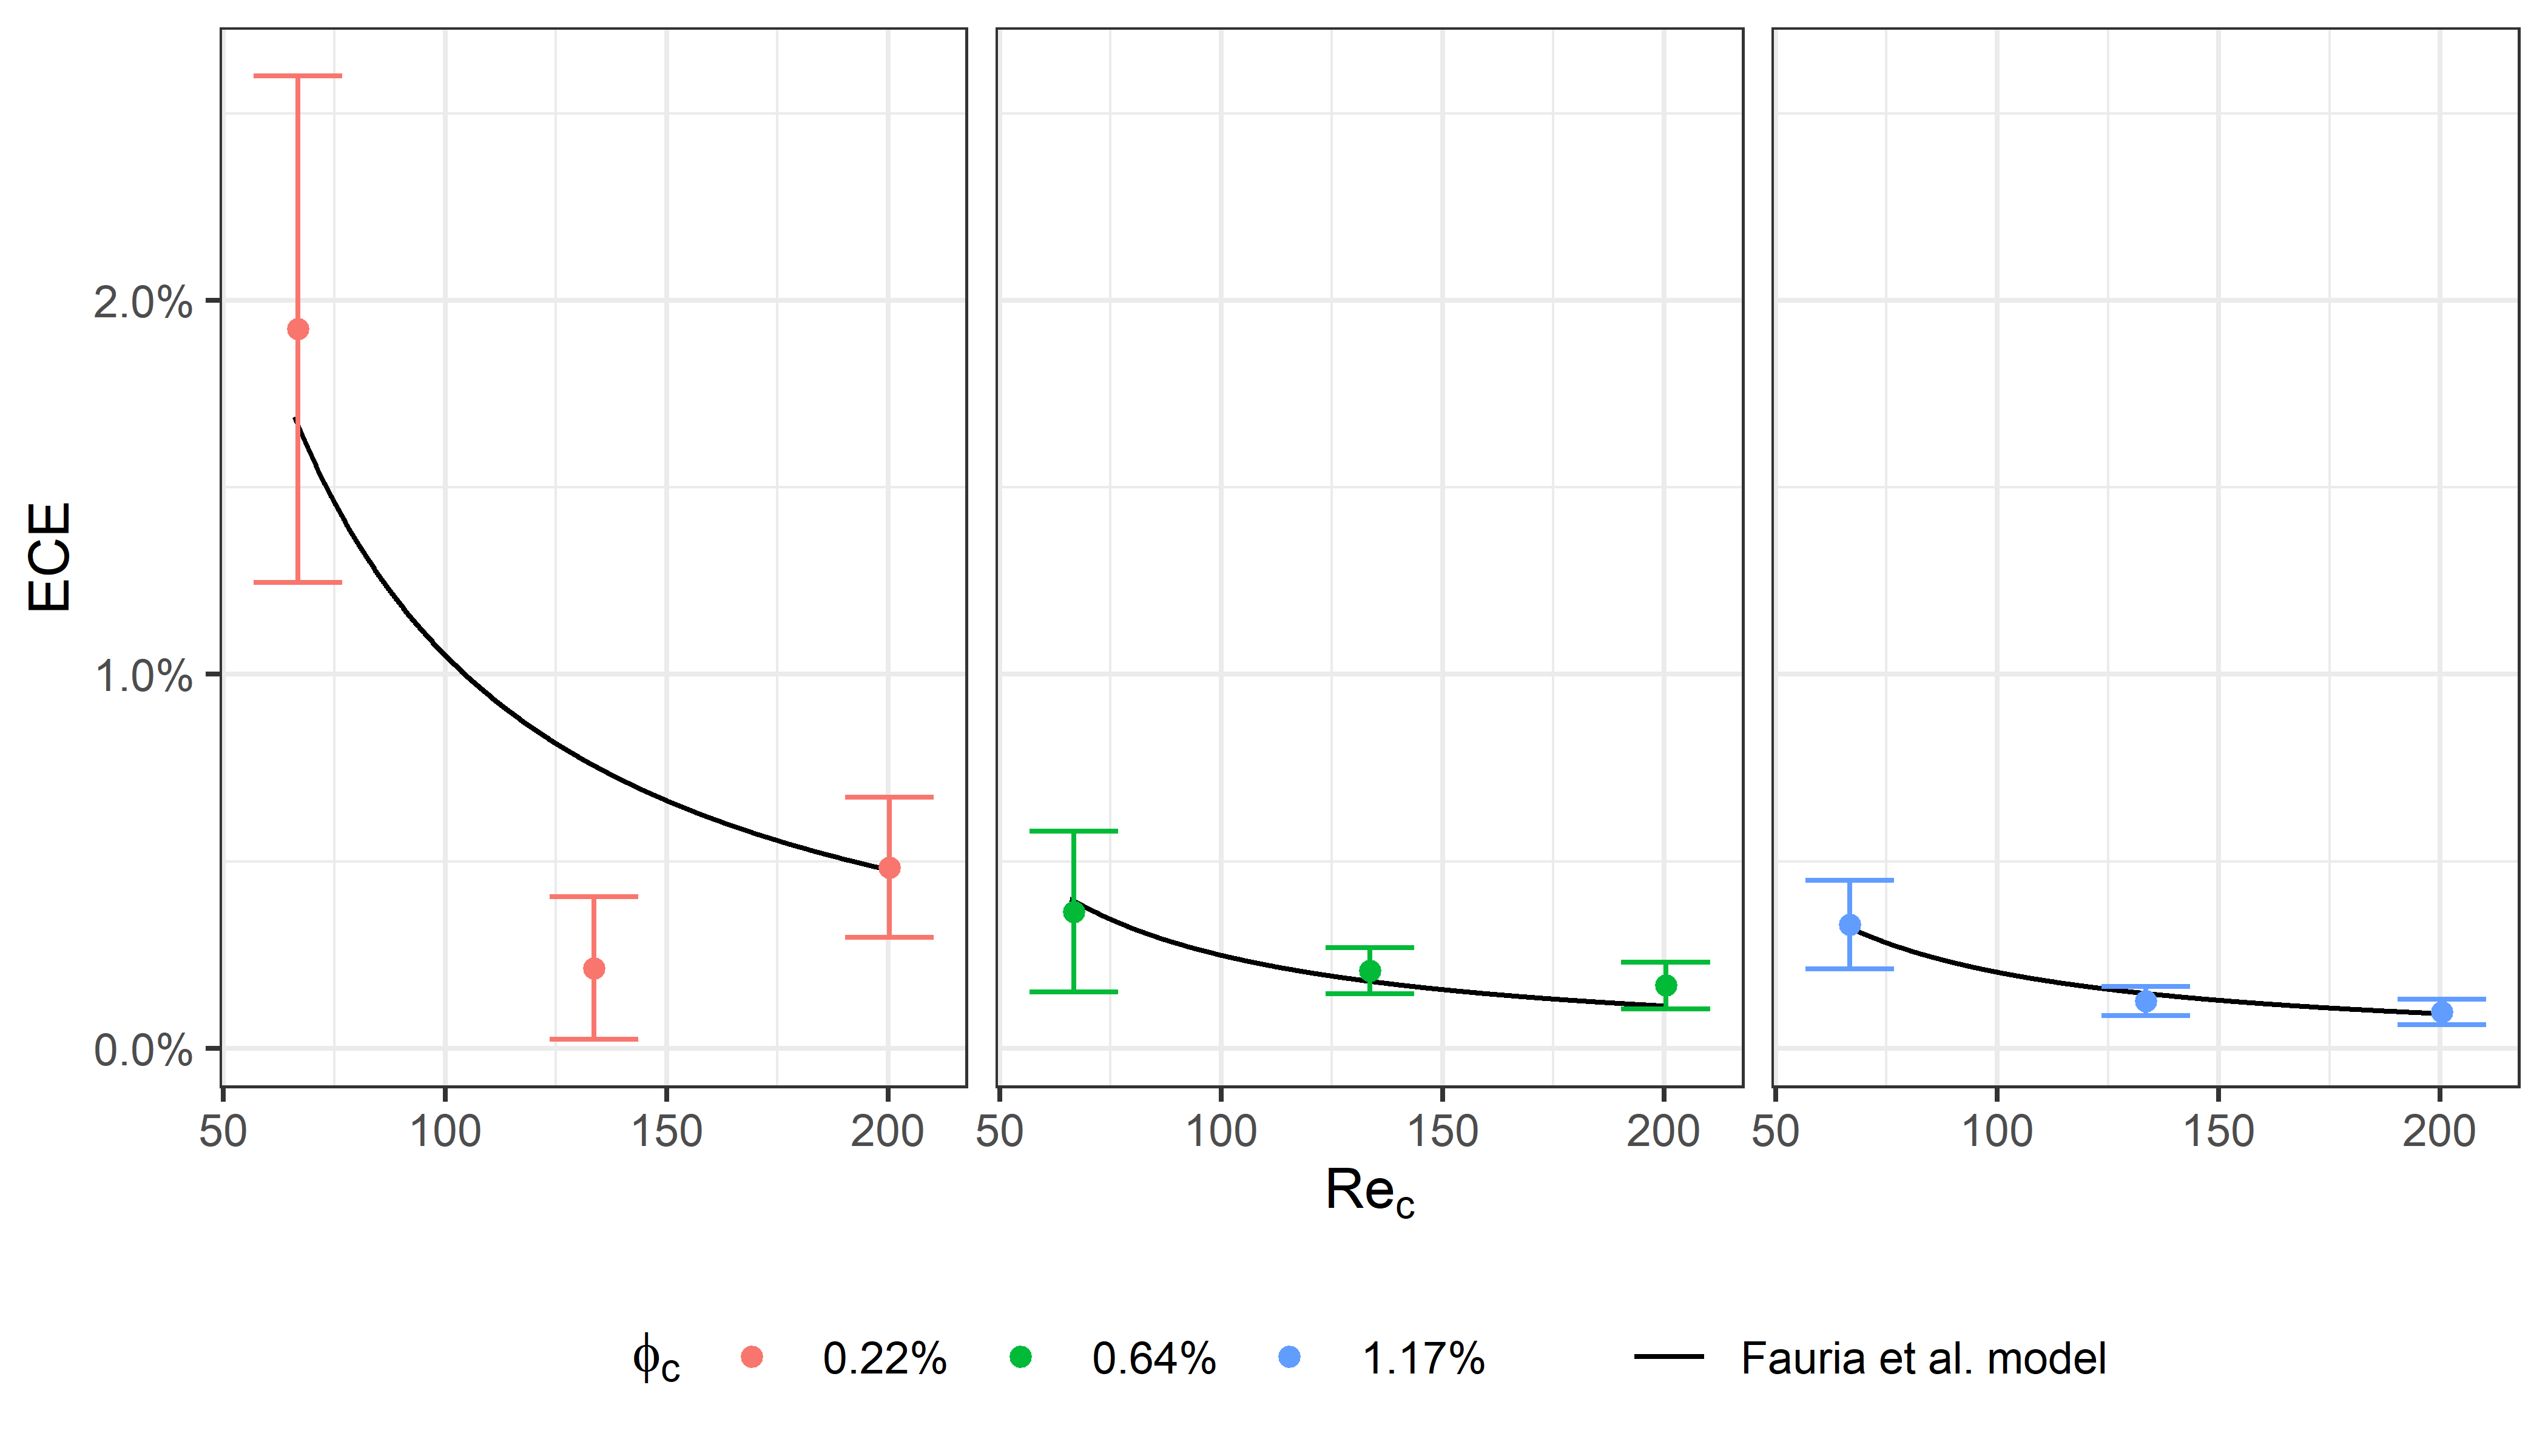
\includegraphics[width=5in]{../pics/comparisonplot.png}
\caption{A comparison of our experimental estimates of effective capture efficiency, colored according to collector solid volume fraction ($\phi_c$), and the predictions of the Fauria et al. \cite{Fauria_2015} power law model (black lines). Effective capture efficiency is plotted on a log scale in order to display model fit more precisely at small values. Error bars represent +/- 1 SE.}
\label{fig:compplot}
\end{figure}   

% C-phi model figure
\begin{figure}[H]
\centering
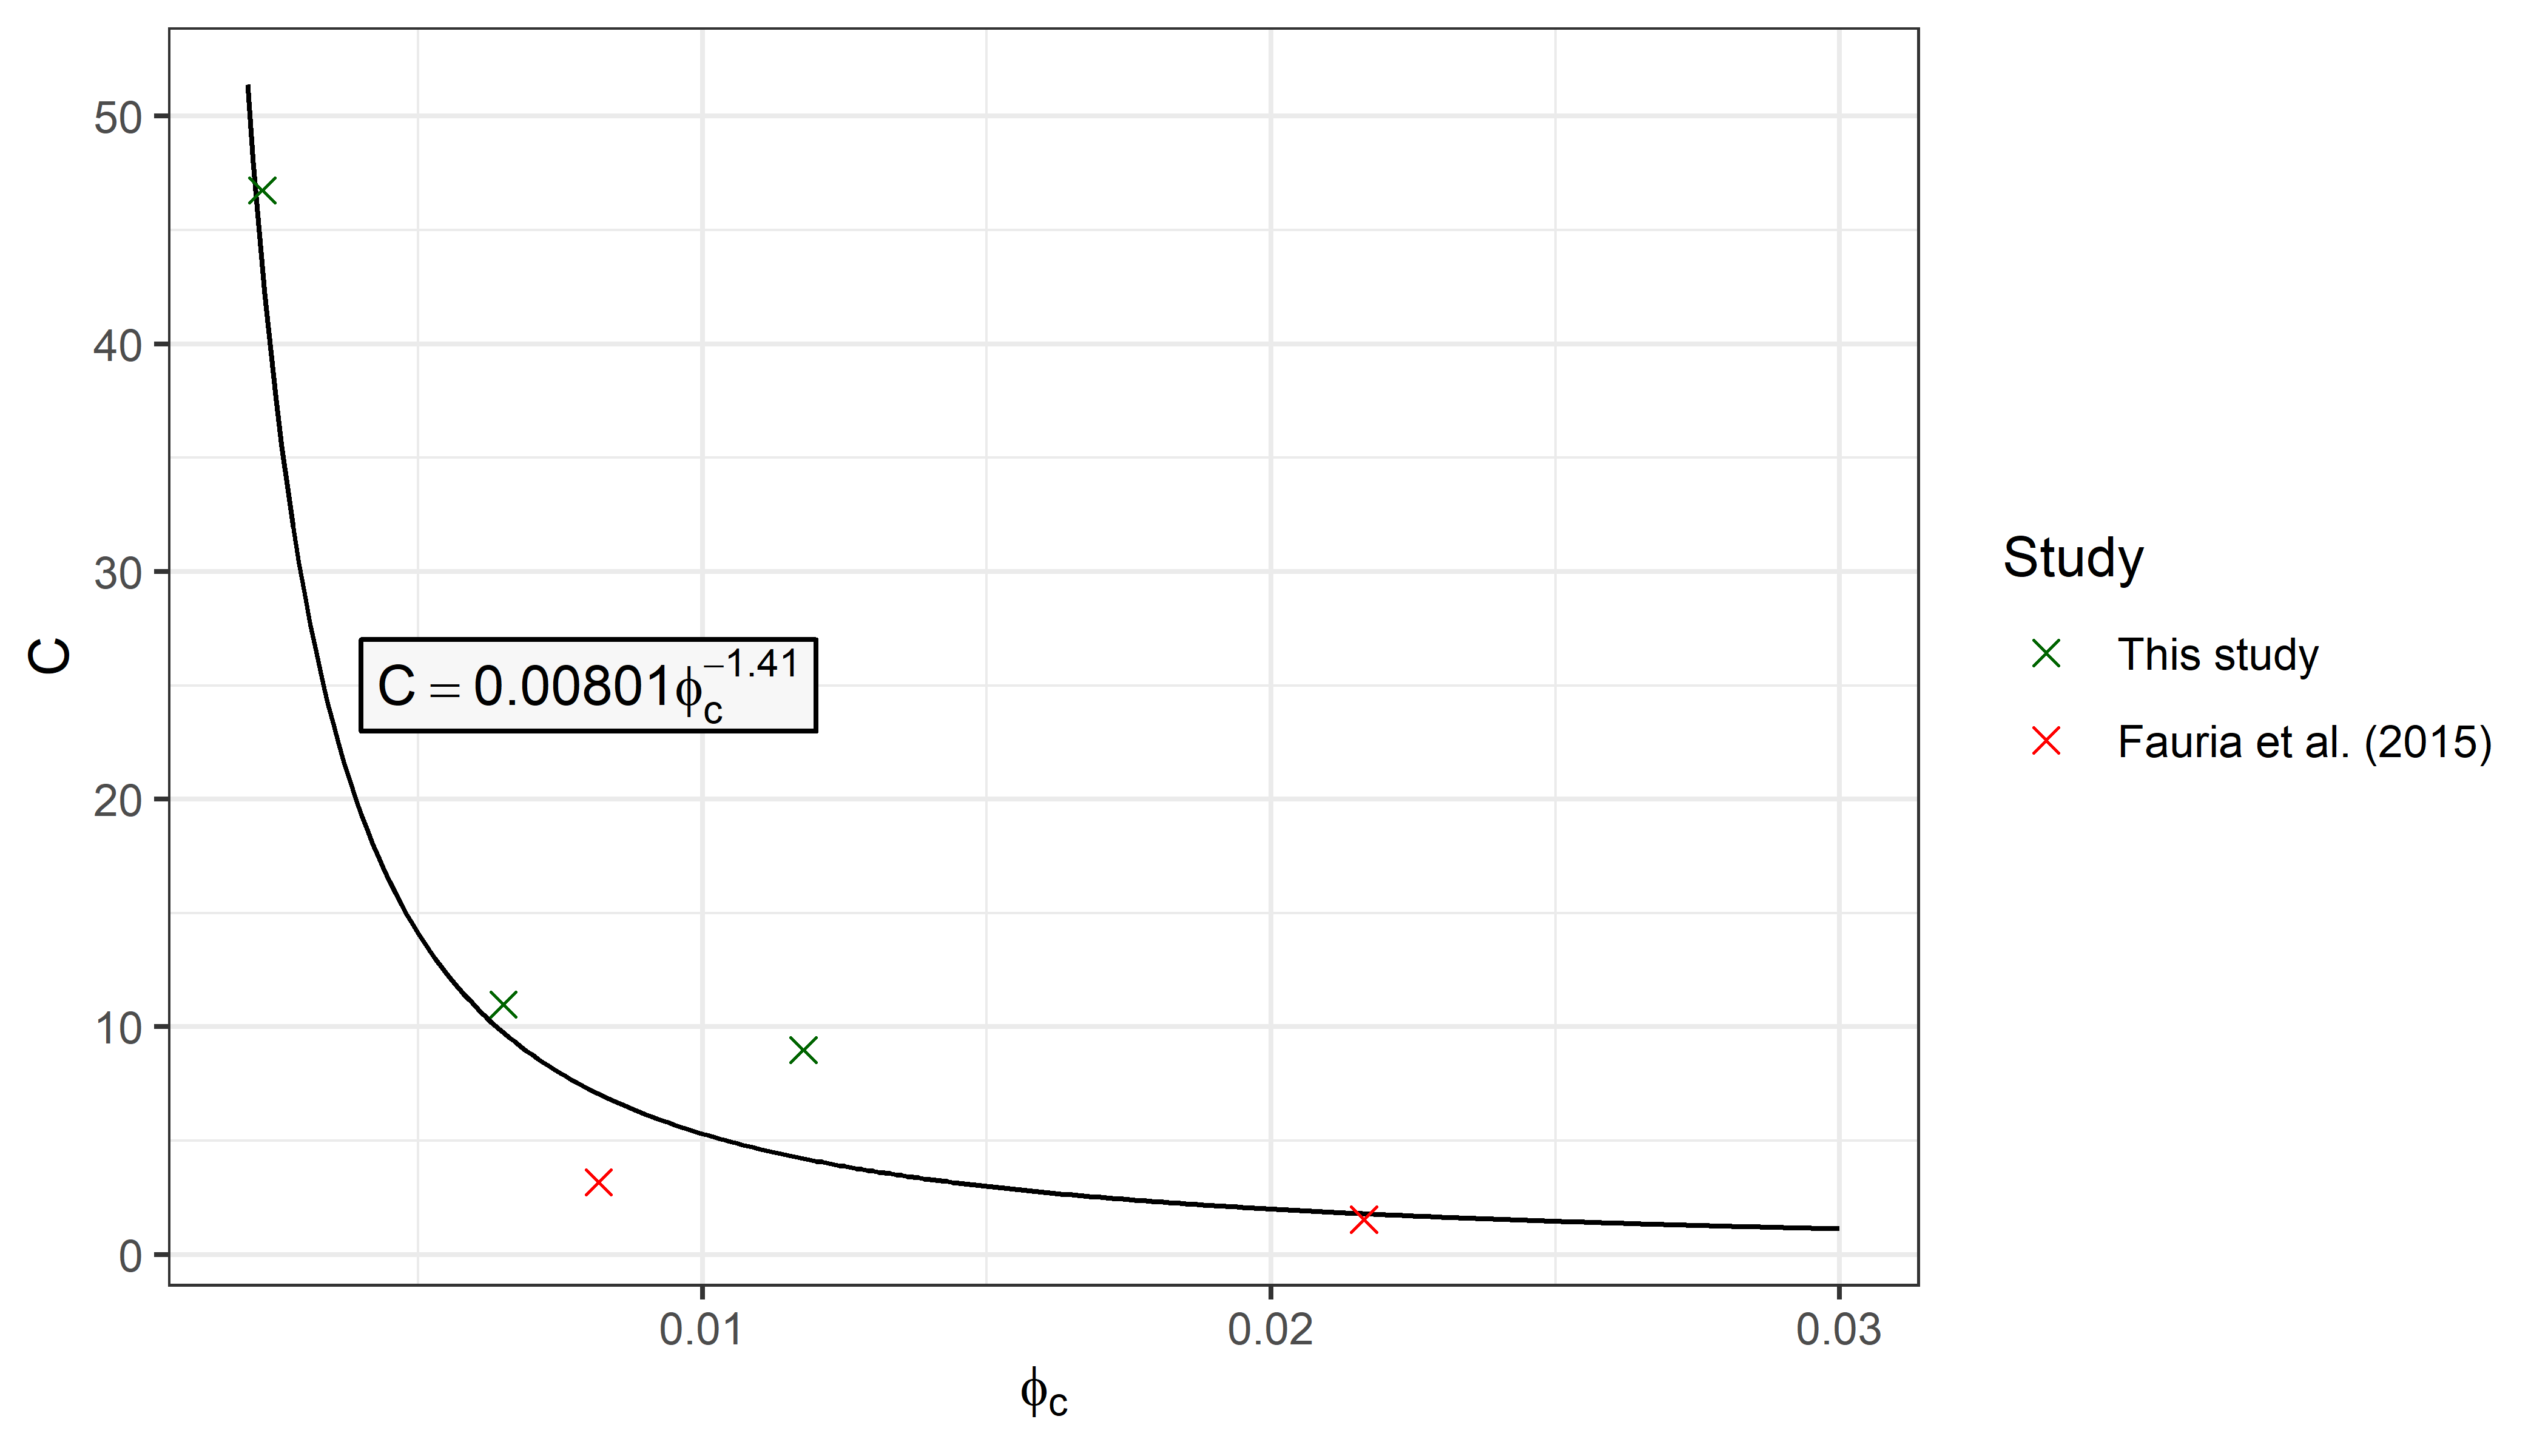
\includegraphics[width=5in]{../pics/cphiplot.png}
\caption{A comparison of the $C$ values calculuated for each of our collector-density treatments to those calculated by Fauria et al. \cite{Fauria_2015}. The black line represents the power-law model of best fit between $C$ and collector solid volume fraction ($\phi_c$) for our collector-density treaments and those of Fauria et al. combined (n = 5), for which R$^2$ = 0.82.}
\label{fig:cphi}
\end{figure}   

The threshold in TKE's relationship with collector density likely indicates that the turbulent eddy scale and the distance between collectors converged somewhere in our parameter space, so that additional collectors acted to damp eddies as much or more than they acted to create them. Accounting for secondary turbulence in future models and experiments seems feasible and important. In general, moving on from the simplistic power-law models developed initially as a way to bridge the gap between analytical expressions for creeping and potential flows to more theoretically-grounded empirical models \cite{stein2020} seems a promising avenue for future investigation.

The ECE of 1.92\% that we observed at our lowest $\Rey_c$ and collector-density treatment is one of the highest observed in any laboratory experiment with multiple collectors \cite{stein2020}. Our observation did fall above the value (1.67\%) predicted by the Fauria et al. model \cite{Fauria_2015} that was fit at that collector density. However, the anomalous experiment at the middle $\Rey_c$ treatment that also influenced that model's fit (Figure \ref{fig:compplot}) probably explains some or all of that difference. Repeating the experiment with the same parameters failed to rectify the anomaly, since it yielded a similar ECE estimate.

On the whole, our results demonstrate that the Fauria et al. model remains a reasonably good predictor of ECE even at collector densities lower than those they studied, and add to the pool of evidence that ECE in settings with multiple stems has a negative relationship with $\Rey_c$ \cite{Fauria_2015,wu2014colloid}, as opposed to the positive relationship between $\eta$ and $\Rey_c$ observed for sediment in settings with only one stem \cite{Palmer_2004}. 

We attribute that difference in part to resuspension driven by turbulent wakes from upstream stems. It is noteworthy that we observed a negative effect despite greasing our stems with the same product and protocol used by Palmer \cite{Palmer_2004}, calling into question previous assumptions that $p_r = 1$ for greased dowels. While Purich \cite{purich2006capture} did empirically confirm resuspension from their greased collectors was low, they did so based on a dowel holding relatively few particles (n = 35). If those particles were added manually before the test, or if they remained on the dowel throughout agitation when others might have been removed, they might not reflect the average resuspension behavior of captured particles.

\subsection{Relative Importance of Biofilm}

The presence of biofilm, which is thought to predominantly affect particle adherence and retention, was found to have a substantial positive effect on ECE. Because Fauria et al. \cite{Fauria_2015} already confirmed that the negative effect of $\Rey_c$ on ECE is supported both with and without biofilm present, and because the duration of growth makes biofilm runs quite time-intensive, we focused solely on collector density's interactions with biofilm. Roughly equivalent biofilm growth (visibly apparent after 13-20 days) resulted in similar relative increase of ECE across our collector density parameter range (improvement to 1.53--2.38 times control), despite quite different absolute values of ECE. As Fauria et al. \cite{Fauria_2015} found for $\Rey_c$, biofilm-positive runs---like biofilm-negative runs---exhibited consistent decline in ECE with increasing collector density.

Absolute effects of biofilm were on par with those of $\Rey_c$ and collector density across our parameter space. At the Reynolds number (200) used for biofilm experiments, ECE ranged from 0.10\% to 0.48\% across our collector-density treatments without biofilm, for an effect size of 0.38\%, and absolute effects of biofilm ranged from +0.07\% ECE to +0.71\% ECE. Absolute effects of $\Rey_c$ (0.20\%--1.71\% ECE) on ECE for specific collector densities were larger than the biofilm effect sizes by a ratio of roughly 2.5:1. This demonstrates biofilm's effect is on the same order of magnitude as the other variables, but the fact that our parameter ranges span a subset of reasonable natural values means that these comparisons should be considered to be inexact.

The multiplicative nature of biofilm's relationship with ECE, and biofilm's apparent importance relative to other factors, makes incorporating quantitative measures of biofilm in future models for ECE seem like a promising avenue. We are unable to do so here because we did not measure biofilm growth quantitatively, aside from our effort to standardize it across treatments of the other variables. To develop such a model, more sophisticated hydroponic equipment to monitor and account for factors impacting growth rate \cite{schnurr2014effect, trulear1982dynamics}, and protocols for measuring the mass and other characteristics of biofilm grown \cite{liu1994simple,characklis1982dynamics}, should be incorporated in future experiments. Additionally, the strands we observed forming on collectors led us to question the relative proportion of capture due to filamentous versus surficial biofilm, another question in need of investigation.

\subsection{Designing Wetlands for Maximum Sedimentation}



\vspace{6pt} 

%%%%%%%%%%%%%%%%%%%%%%%%%%%%%%%%%%%%%%%%%%
%% optional
\supplementary{The following are available online at \linksupplementary{s1}, Figure S1: title, Table S1: title, Video S1: title.}

% Only for the journal Methods and Protocols:
% If you wish to submit a video article, please do so with any other supplementary material.
% \supplementary{The following are available at \linksupplementary{s1}, Figure S1: title, Table S1: title, Video S1: title. A supporting video article is available at doi: link.}

\authorcontributions{Conceptualization, L.L., J.N., and J.W.; methodology, L.L. and J.W.; software, L.L., J.N., J.W., and C.Y.; validation, J.W.; formal analysis, J.W. and C.Y.; investigation, J.N., J.W, and C.Y.; resources, L.L.; data curation, J.W.; writing--original draft preparation, J.N., J.W., and C.Y.; writing--review and editing, L.L., J.N., J.W., and C.Y.; visualization, J.W.; supervision, L.L., J.W., and C.Y.; project administration, L.L. and J.W.; funding acquisition, L.L.}

\funding{This research was funded by NSF award \#1455362.}

\acknowledgments{The authors wish to thank and acknowledge Colin Keating and Aaron Hurst for their helpful work on preliminary flume experiments. We also wish to express great thanks to Yayla Sezginer, Elle Chen, Nicole Ulakovic, Katrina Ginsberg, and Danielle Satin for their time spent preparing for experiments, maintaining the flume, and fastidiously carrying out other important laboratory tasks. Lastly, we wish to thank Sam Stein and Sheila Trampush for graciously sharing data and participating in brainstorming sessions while working on concurrent studies within the same general topic area.}

\conflictsofinterest{The authors declare no conflict of interest.} 

%% optional
 \abbreviations{The following notations are used in this manuscript:
 
 \noindent \begin{tabular}{@{}ll}
 $\eta$ & particle capture efficiency, dimensionless\\
 $w_u$ & upstream width of streamlines that intersect a collector, cm\\
 $d_c$ & collector diameter, cm\\
 $\eta^\prime$ & effective capture efficiency (ECE), dimensionless\\
 $p_r$ & probability of particle retention, dimensionless \\
 $d_p$ & particle diameter, \SI{}{\micro\metre} \\
 $\Rey_c$ & collector Reynolds number, dimensionless \\
 $u$ & flow velocity, cm/s \\
 $\nu$ & kinematic viscosity \SI{}{\centi\metre\squared/\second} \\
 $R$ & particle-collector diameter ratio, dimensionless \\
 $C,a,b$ & power-law coefficients (Eq. (\ref{eq:powerlaw})), dimensionless \\
 $N_\Pec$ & Peclet number, dimensionless \\
 $\bar{\phi}$ & depth-averaged suspended sediment concentration, \SI{}{\micro\liter/\liter} \\
 $t$ & time, s \\
 $h$ & water depth, cm \\
 $z$ & height above the bed, cm \\
 $\phi_z$ & suspended sediment concentration at height $z$, \SI{}{\micro\liter/\liter} \\
 $k_s$ & concentration time-decay due to settling, s$^{-1}$ \\
 $v_s$ & settling velocity, cm/s \\
 $C_b$ & constant relating near-bed concentration to depth-averaged concentration, dimensionless \\
 $E_r$ & entrainment rate, dimensionless \\
 $k_c$ & concentration time-decay due to capture, s$^{-1}$ \\
 $I_c$ & collector height density, \SI{}{\metre/\metre\cubed} \\
 $N_c$ & number of collectors, \# \\
 $V$ & test-section water volume, \SI{}{\metre\cubed} \\
 $z_r$ & reference height (Eq. (\ref{eq:rouse})), cm \\
 $\phi_r$ & suspended sediment concentration at reference height $z_r$, \SI{}{\micro\liter/\liter} \\
 $R_0$ & Rouse number, dimensionless \\
 $m_s$ & sediment mass settled in test section, g \\
 $m_0$ & sediment mass suspended at beginning of experiment, g \\
 $T$ & total duration of experiment, s \\
 $k_b$ & background concentration time-decay, s$^{-1}$ \\
 $\phi_c$ & collector solid volume fraction, dimensionless
 \end{tabular}}

%%%%%%%%%%%%%%%%%%%%%%%%%%%%%%%%%%%%%%%%%%
%% optional
\appendixtitles{yes} %Leave argument "no" if all appendix headings stay EMPTY (then no dot is printed after "Appendix A"). If the appendix sections contain a heading then change the argument to "yes".
\appendix
\section{Secondary methodology}
\unskip
\subsection{Particle Size}
\begin{figure}[H]
\centering
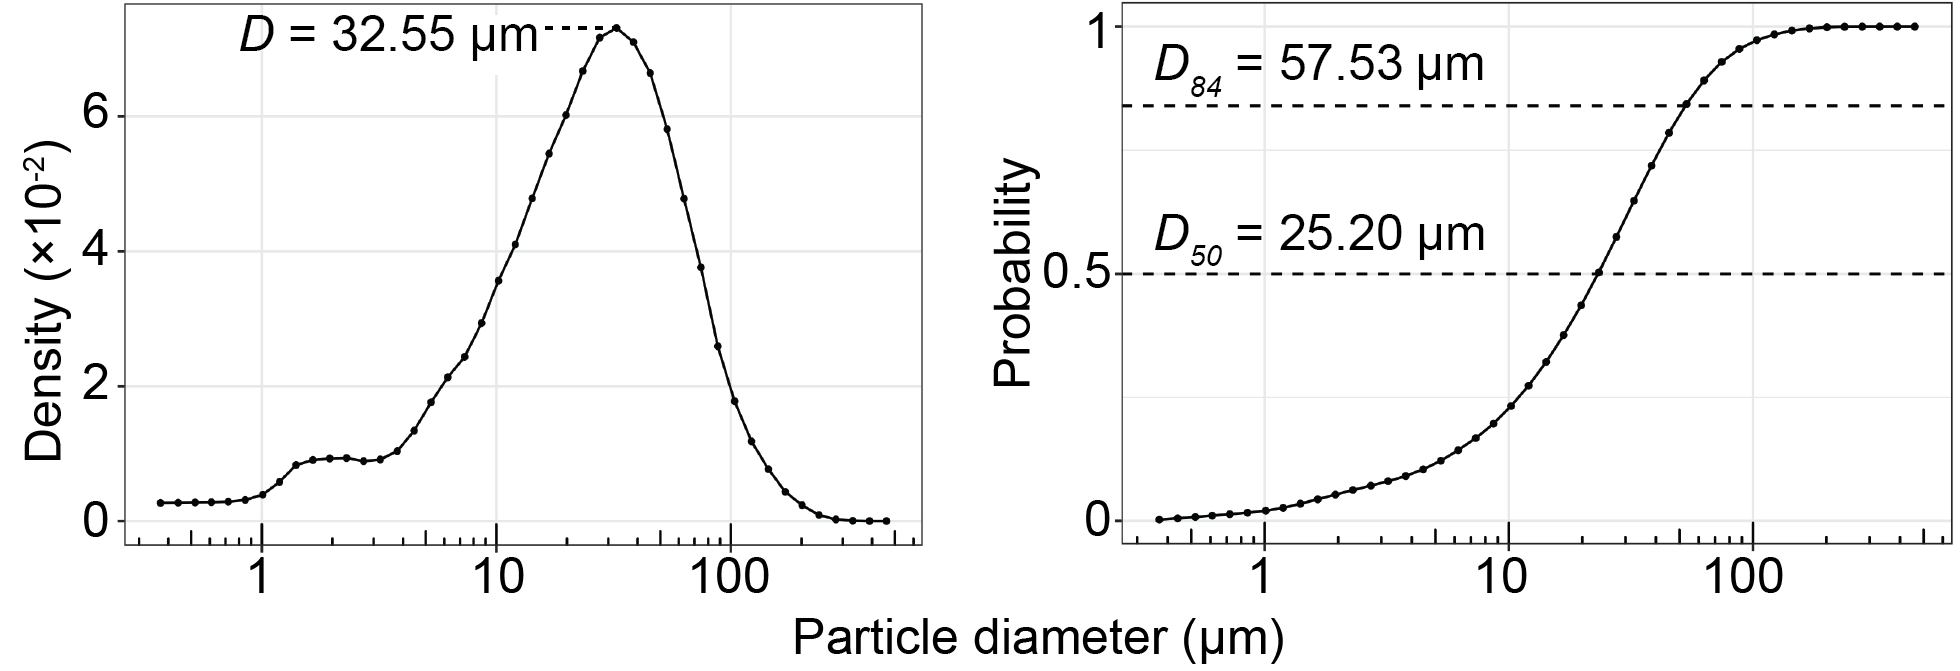
\includegraphics[width=5in]{../pics/wf5-200sizedist.png}
\caption{Walnut shell flour (WF5-200) particle size distribution, as measured by LISST-XR|Portable. (\textbf{a}) Probability density function, with mode (\SI{32.55}{\micro\metre}) indicated. (\textbf{b}) Cumulative density function, with 50th (\SI{25.20}{\micro\metre}) and 84th (\SI{57.53}{\micro\metre}) percentiles highlighted.}
\end{figure}

\subsection{Flume Volume}

In order to estimate ECE, we need to know the particle capture rate for water that is being acted upon by the collectors (i.e., in the test section). This requires scaling up by the ratio between the test section volume (1.95 m $\times$ 0.6 m $\times$ 0.4 m = \SI{0.468}{m^3}) and the water volume of the flume's entire wetted floorplan under experimental conditions (depth = 0.4 m in test section). Because of the flume's irregular floorplan and shape, estimating its water volume theoretically is impractical, and technical documents were calculated at a different water depth, so we made an empirical estimate. 

We drained the flume after an experiment while measuring flow rate at the drain outlet over time, performed polynomial regression (Figure \ref{fig:flumevol}), and calculated a definite integral ($V = \int_{t_{full}}^{t_{empty}}{-\frac{dV}{dt}dt}$) from when draining began to when the part of the flume involved in the experimental flows was empty . Because polynomials of second order and above fit well and yielded very similar volume estimates, we felt confident using \SI{2.43}{\metre\cubed} as the flume volume in our calculations (Table \ref{tbl:flumevol}).


\begin{figure}[H]
\centering
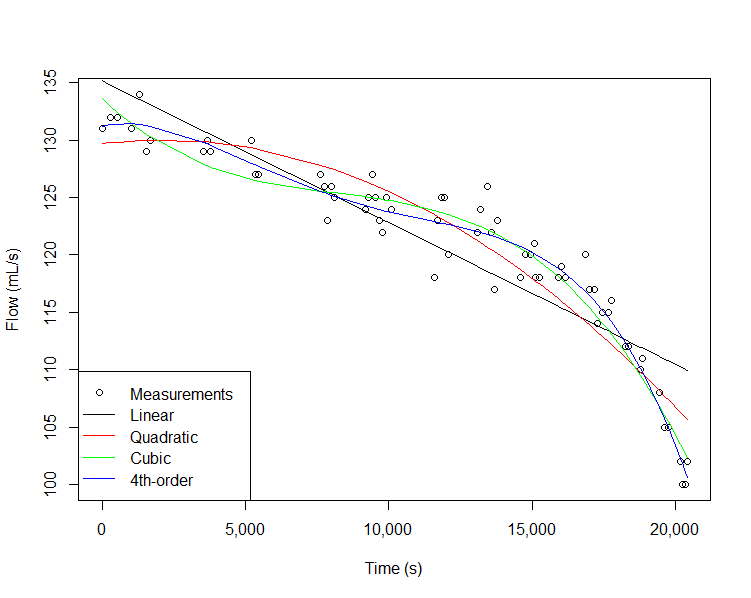
\includegraphics[width=4.7in]{../pics/flumevol.png}
\caption{Polynomial models predicting the rate at which the flume drained, to be integrated to estimate the volume in circulation during experiments.}
\label{fig:flumevol}
\end{figure}

\begin{table}[H]
\caption{Polynomial model summary}
\centering
%% \tablesize{} %% You can specify the fontsize here, e.g., \tablesize{\footnotesize}. If commented out \small will be used.
\begin{tabular}{lrr}
\toprule
\textbf{Model}&\textbf{Estimated Volume (\SI{}{\metre\cubed})}&\textbf{R$^2$}\\
\midrule
Linear       &  2.4309     &   0.80\\
Quadratic    &  2.4277     &   0.90\\
Cubic        &  2.4373     &   0.94\\
4th-order    &  2.4294     &   0.96\\
\bottomrule
\label{tbl:flumevol}
\end{tabular}
\end{table}

\subsection{Heteroskedasticity Reduction}

Because measurement error was proportional to sample concentration, which was greater at the beginning of experiments than at the end, heteroskedasticity was observed in our suspended concentration data. We log-transformed the data and then performed linear regression, confirming that heteroskedasticity was reduced in comparison to least-squares exponential regression on the raw data (Figure \ref{fig:heterosked}). While it would be preferable to also address non-randomness (i.e., curvature) in the residuals \textit{post hoc}, subsetting data across time is not advisable because $k_s$ was calculated for $T$, the total run duration.

\begin{figure}[H]
\centering
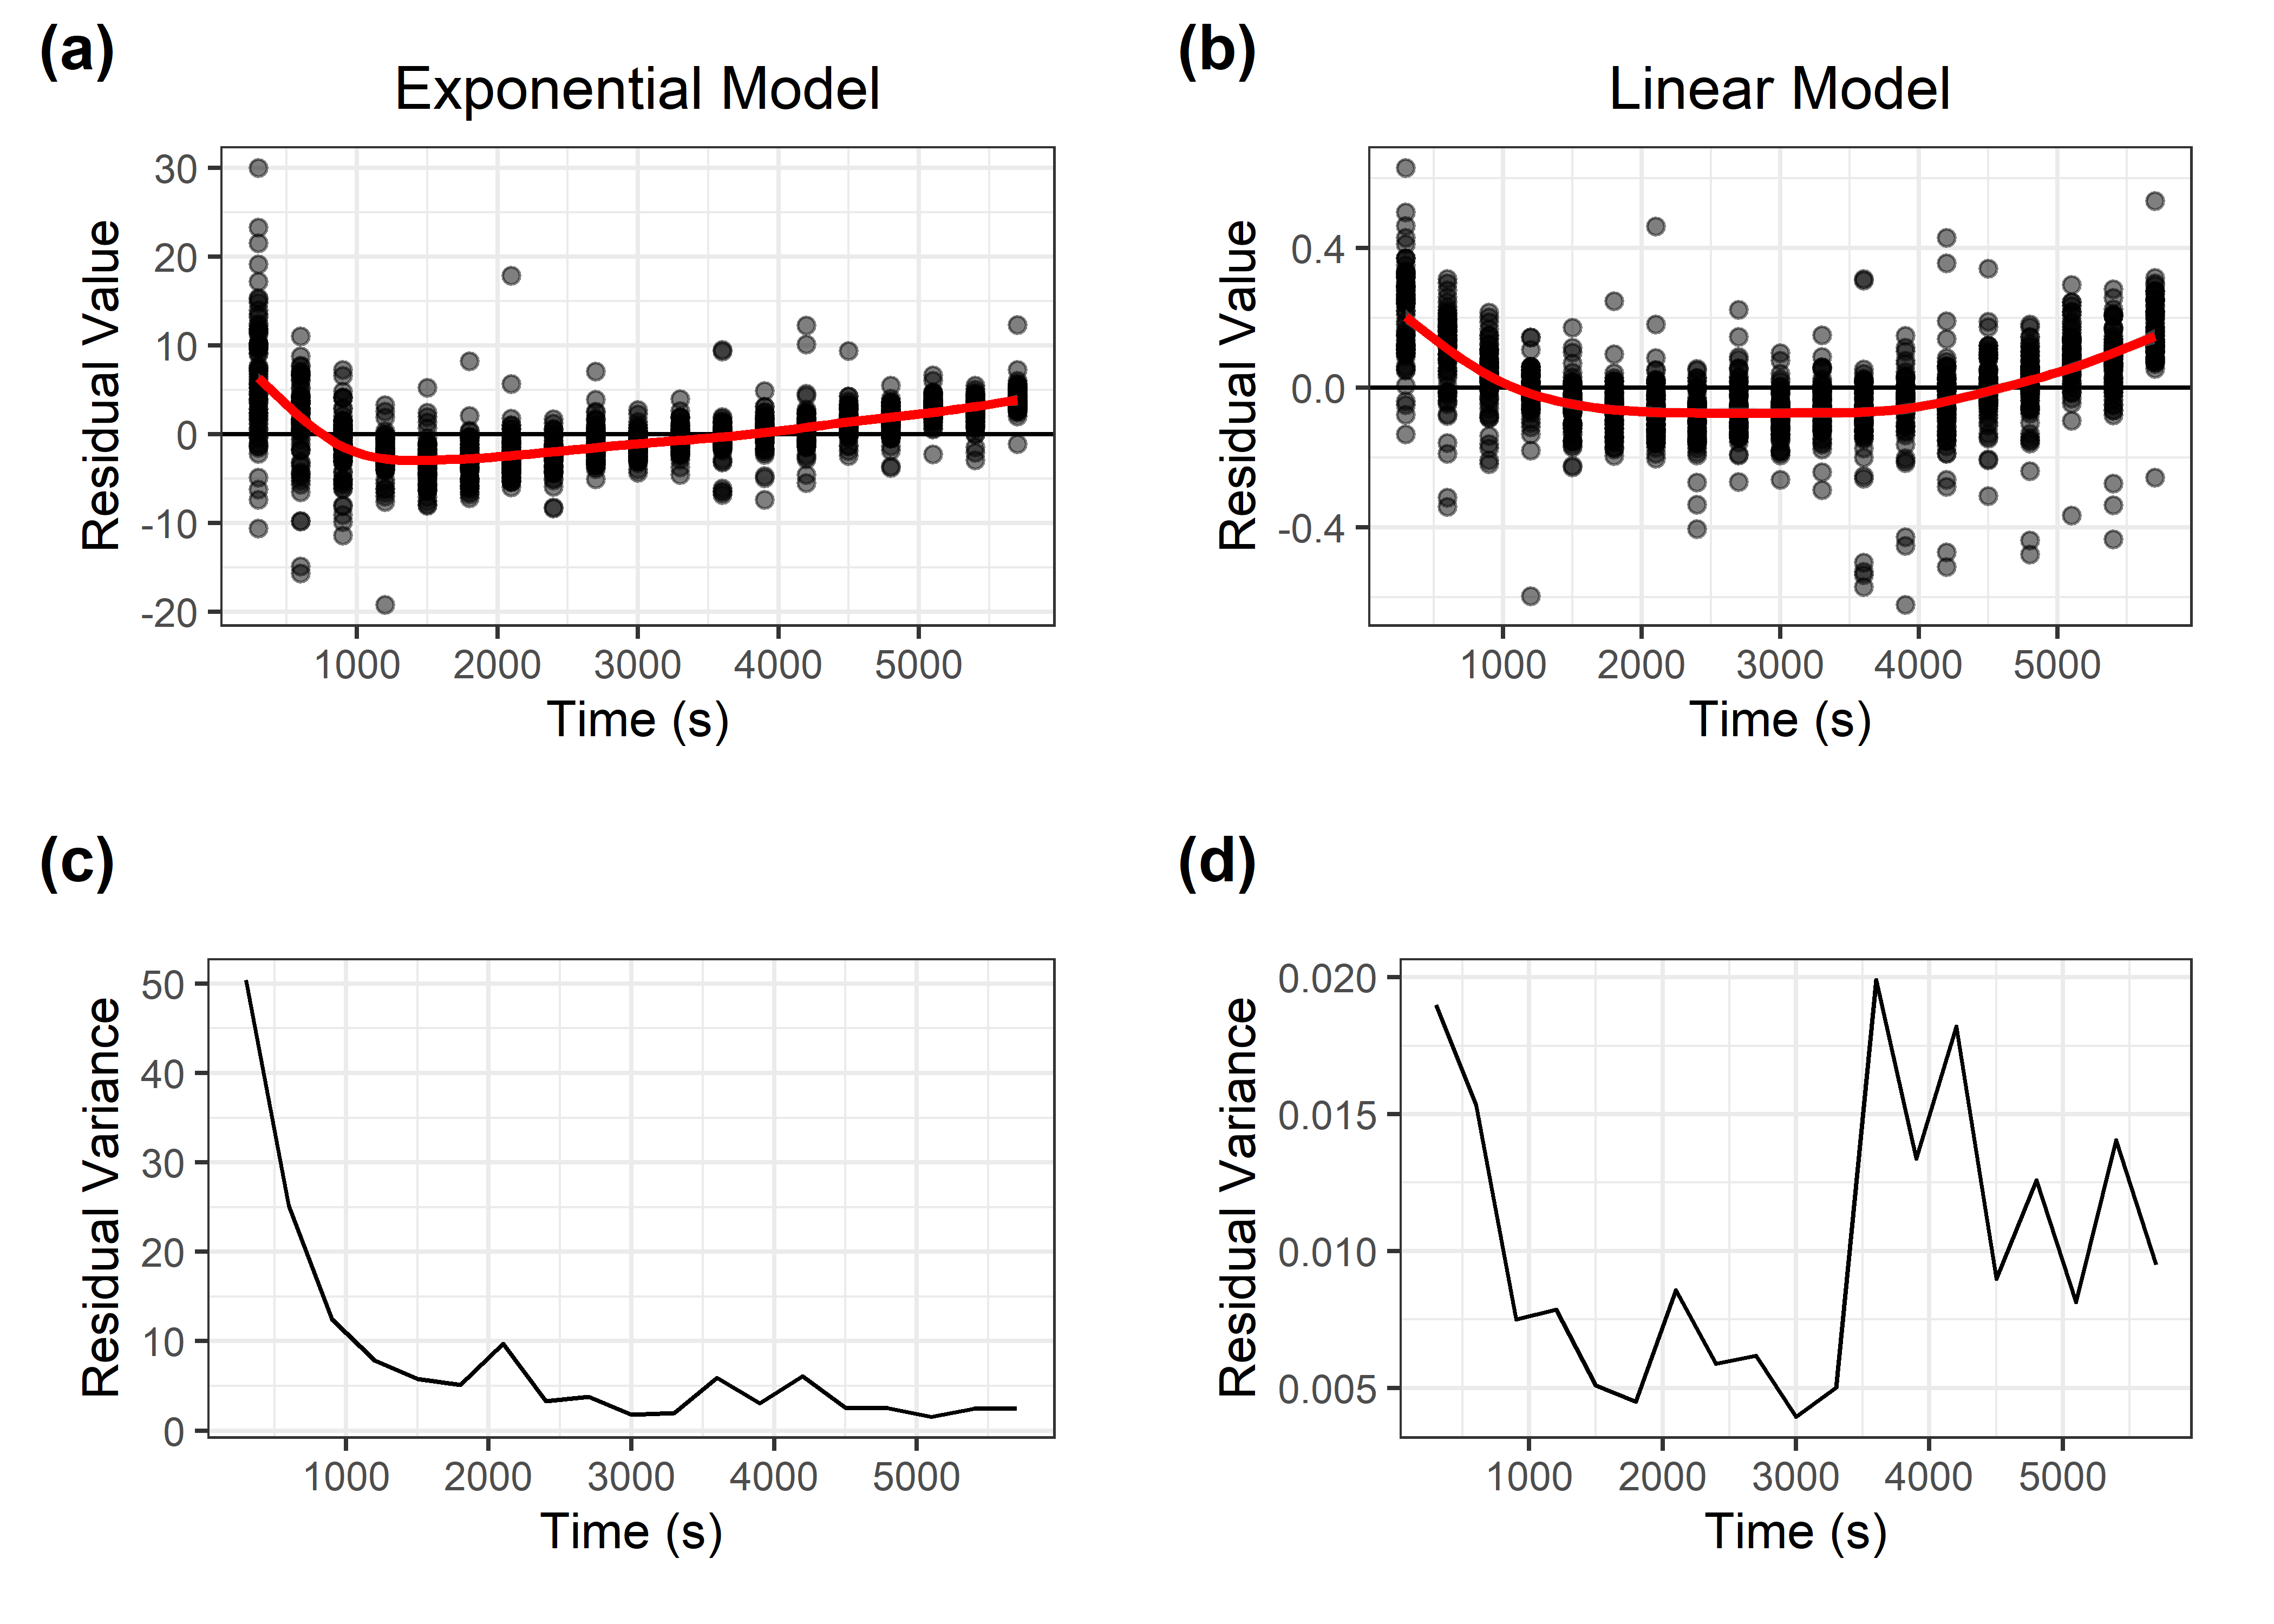
\includegraphics[width=5.5in]{../pics/heterosked.png}
\caption{Plots of residuals and residual variance pooled from all 12 experimental treatments including controls. Red lines are locally-weighted smoothing functions \textbf{(a)} Residuals of the exponential model. \textbf{(b)} Residuals of the transformed linear model used in analyses. \textbf{(c)} Variance of the residual values of the exponential model. \textbf{(d)} Variance of the residual values of the linear model used in analyses.}
\label{fig:heterosked}
\end{figure}

%%%%%%%%%%%%%%%%%%%%%%%%%%%%%%%%%%%%%%%%%%
% Citations and References in Supplementary files are permitted provided that they also appear in the reference list here. 

%=====================================
% The following MDPI journals use author-date citation: Arts, Econometrics, Economies, Genealogy, Humanities, IJFS, JRFM, Laws, Religions, Risks, Social Sciences. For those journals, please follow the formatting guidelines on http://www.mdpi.com/authors/references
% To cite two works by the same author: \citeauthor{ref-journal-1a} (\citeyear{ref-journal-1a}, \citeyear{ref-journal-1b}). This produces: Whittaker (1967, 1975)
% To cite two works by the same author with specific pages: \citeauthor{ref-journal-3a} (\citeyear{ref-journal-3a}, p. 328; \citeyear{ref-journal-3b}, p.475). This produces: Wong (1999, p. 328; 2000, p. 475)

% =====================================
% References, variant B: external bibliography
% =====================================

\reftitle{References}

\externalbibliography{yes}

\bibliography{refs}

%%%%%%%%%%%%%%%%%%%%%%%%%%%%%%%%%%%%%%%%%%
%% optional
%\sampleavailability{Samples of the compounds ...... are available from the authors.}

%% for journal Sci
%\reviewreports{\\
%Reviewer 1 comments and authors’ response\\
%Reviewer 2 comments and authors’ response\\
%Reviewer 3 comments and authors’ response
%}

%%%%%%%%%%%%%%%%%%%%%%%%%%%%%%%%%%%%%%%%%%

\noindent \end{document}
